\documentclass[a4paper]{article}

\usepackage{INTERSPEECH2018}
\usepackage{tikz}
\usepackage{url}
\usepackage{blindtext}
\usetikzlibrary{shapes,shadows,arrows,positioning}

\tikzstyle{block} = [draw, fill=white, rectangle, 
    minimum height=3em, minimum width=6em, rounded corners, drop shadow]
\tikzstyle{sum} = [draw, fill=white, circle, node distance=1cm]
\tikzstyle{input} = [coordinate]
\tikzstyle{output} = [coordinate]
\tikzstyle{pinstyle} = [pin edge={to-,thin,black}]

\title{Towards pathological speech synthesis from articulation}
\name{Bence Halpern$^1$$^2$, Rob J. J. H. van Son$^1$, Michiel W. M.
  van den Brekel$^1$$^2$}
%The maximum number of authors in the author list is twenty. If the number of contributing authors is more than twenty, they should be listed in a footnote or in acknowledgement section, as appropriate.
\address{
  $^1$NKI-AVL, Amsterdam\\
  $^2$ACLC, University of Amsterdam, The Netherlands}
\email{b.halpern@nki.nl, r.v.son@nki.nl}

\begin{document}

\maketitle
% 
\begin{abstract}

  This paper presents a technique to synthetise speech that is pathological on the articulation level.
  The technique presented considers a vocoder combined with a speaker-independent articulatory to acoustic neural network using electromagnetic articulography recordings from the three largest articulatory datasets. A speech language pathologist indicated that the synthetised samples reflect some qualities of disordered speech. A visualisation technique is also described to shed light on what these neural networks learn. Further directions are pointed out on how to improve speech quality.
\end{abstract}
\noindent\textbf{Index Terms}: computational paralinguistics, articulatory-to-acoustic
speech synthesis, deep learning, pathological speech

\section{Introduction}

At first, the application of pathological speech synthesis might be unclear to the reader.
However, this area could have many
potential applications. One of them is the creation of synthetic data which could be
used as training data for pathological speech detection. It could be also used as a
clinical tool for counselling patients about post-operative outcomes. Additionally, a
deeper understanding of the articulatory to speech relationship could offer improvement
in speech therapy tools.

Understanding how articulation affects speech is a central question in speech
research. The source-filter model was one of the first models to tackle this
problem by discovering that speech production could be described by
the geometry of the vocal tract and the glottal wave \cite{Benesty2009} \cite{Fant1981}.
A significant drawback of this method however is that it does not model the movement of articulators.

Recently, deep learning methods became popular
to model articulation. These methods use a measurement tool,
called electromagnetic articulography (EMA) to obtain articulation data 
\cite{Aryal2016} \cite{Taguchi} \cite{Liu2018} along with recurrent
neural networks, which are function approximators that are able to deal with
the sequential nature of data \cite{Hochreiter1997}. Data-driven methods became of interest also
in real-time speech synthesis, using a technique called permanent magnetic articulography
by \cite{Gonzalez2017}, resulting in intelligeble
speech.

The conclusion of these endeavours were that while it is possible to
predict some of the pitch from articulation, the quality suffers.
However, it is possible to obtain satisfactory values for the
cepstrum.

This indicates, that this technique could be a good candidate for synthetising
pathological speech where the pitch of the voice is natural. For example,
in the case of tongue cancer speech, the laryngeal function remains intact,
meaning the pitch remains natural. Thus, it is proposed that the \( F_0 \) could
be simply obtained through vocoder analysis and only predict the cepstral
values through articulation to model pathologies.

In this paper, a technique is described which combines healthy speech
from the three largest articulatory datasets, MNGU0 \cite{Richmond2011},
MOCHA-TIMIT and TORGO \cite{Rudzicz2012} for the first time, in order to
create a general speaker-independent articulatory to acoustic model and
introduce a novel framework for pathological speech synthesis.

\vspace{0.5em}
The main contributions of this paper are,
\begin{itemize}
\setlength\itemsep{-0.3em}
\item a description of a method for speaker-independent MFCC prediction in Section \ref{section:method}
\item a technique to incorporate articulation domain-knowledge into pathological
  speech synthesis in Section \ref{section:speech} 
\item a discussion of the current limitations of this framework in Section \ref{section:limitations}
\item an attempt to shed light on what these neural networks might learn in Section \ref{section:visualisation}
\end{itemize}

The research code is also available as a Github repository online. \cite{Halpern2019}

\section{Method} \label{section:method}
\subsection{Dataset preprocessing}

\subsubsection{Electrode preprocessing}

Articulators recorded are slightly different, meaning particular attention has to be paid to align these datasets. An example of EMA recording locations are shown on Figure \ref{fig:electrodes}. Seven electrodes were used for this experiment out of the total eight, Table \ref{tab:electrodes} includes
the alignment of the channels that were used. This ensures that each
input channel records reasonably similar information, meaning that the
channels should have similar variance. These are then standardised on a per speaker
basis. These steps alleviate some
of the speaker-wise deviations, but does not alleviate problems if an electrode
falls off during the experiment or if an electrode needs to be changed.

In the case of the TORGO dataset, some of the channels contained artifacts,
these have been excluded. The signal to noise
ratio in these spiky regions was low enough to affect
training.

Previously \cite{Gonzalez2016}, the effect of delay on the
output signal were investigated. It has been found that delay
is beneficial for the case of causal models. In Section \ref{section:nnexperiment},
a bidirectional recurrent model will be introduced which is not causal, meaning there is no need for delays.

\begin{table}[th]
  \caption{Articulatory information recorded in datasets}
  \label{tab:electrodes}
  \centering
  \begin{tabular}{ r r r  }
    \toprule
    \textbf{MNGU0} & \textbf{MOCHA-TIMIT} & \textbf{TORGO} \\ 
    \midrule
    Tongue dorsum (T3) & Tongue dorsum (T3) & Tongue back \\
    Tongue blades (T2) & Tongue blades (T2) & Tongue middle \\
    Tongue tip (T1) & Tongue tip (T1) & Tongue tip \\
    Lower incisor (T3) & Jaw & Lower incisor\\
    Upper incisor & Nose & Upper incisor\\
    Upper lip & Upper lip & Upper lip \\
    Lower lip & Lower lip  & Lower lip\\
    \bottomrule
    \end{tabular}
\end{table}


\begin{figure}[t]
  \caption{The visualisation of electrode locations for 300 samples from
    the MNGU0 dataset at their initial position.}
  \label{fig:electrodes}
  \begin{center}
    \scalebox{0.50}{\input{init_pos.pgf}}
\end{center}
\end{figure}

\begin{figure}[t]
  \caption{Thresholded Prewitt mask of activations indicates that a boundary phenomena is learned by the neural network. Best viewed in zoom.}
  \label{fig:mask}
  \begin{center}
    \scalebox{0.40}{%% Creator: Matplotlib, PGF backend
%%
%% To include the figure in your LaTeX document, write
%%   \input{<filename>.pgf}
%%
%% Make sure the required packages are loaded in your preamble
%%   \usepackage{pgf}
%%
%% Figures using additional raster images can only be included by \input if
%% they are in the same directory as the main LaTeX file. For loading figures
%% from other directories you can use the `import` package
%%   \usepackage{import}
%% and then include the figures with
%%   \import{<path to file>}{<filename>.pgf}
%%
%% Matplotlib used the following preamble
%%   \usepackage{fontspec}
%%   \setmainfont{DejaVu Serif}
%%   \setsansfont{DejaVu Sans}
%%   \setmonofont{DejaVu Sans Mono}
%%
\begingroup%
\makeatletter%
\begin{pgfpicture}%
\pgfpathrectangle{\pgfpointorigin}{\pgfqpoint{8.200000in}{8.200000in}}%
\pgfusepath{use as bounding box, clip}%
\begin{pgfscope}%
\pgfsetbuttcap%
\pgfsetmiterjoin%
\definecolor{currentfill}{rgb}{1.000000,1.000000,1.000000}%
\pgfsetfillcolor{currentfill}%
\pgfsetlinewidth{0.000000pt}%
\definecolor{currentstroke}{rgb}{1.000000,1.000000,1.000000}%
\pgfsetstrokecolor{currentstroke}%
\pgfsetdash{}{0pt}%
\pgfpathmoveto{\pgfqpoint{0.000000in}{0.000000in}}%
\pgfpathlineto{\pgfqpoint{8.200000in}{0.000000in}}%
\pgfpathlineto{\pgfqpoint{8.200000in}{8.200000in}}%
\pgfpathlineto{\pgfqpoint{0.000000in}{8.200000in}}%
\pgfpathclose%
\pgfusepath{fill}%
\end{pgfscope}%
\begin{pgfscope}%
\pgfsetbuttcap%
\pgfsetmiterjoin%
\definecolor{currentfill}{rgb}{1.000000,1.000000,1.000000}%
\pgfsetfillcolor{currentfill}%
\pgfsetlinewidth{0.000000pt}%
\definecolor{currentstroke}{rgb}{0.000000,0.000000,0.000000}%
\pgfsetstrokecolor{currentstroke}%
\pgfsetstrokeopacity{0.000000}%
\pgfsetdash{}{0pt}%
\pgfpathmoveto{\pgfqpoint{0.579340in}{4.336458in}}%
\pgfpathlineto{\pgfqpoint{4.073386in}{4.336458in}}%
\pgfpathlineto{\pgfqpoint{4.073386in}{7.966667in}}%
\pgfpathlineto{\pgfqpoint{0.579340in}{7.966667in}}%
\pgfpathclose%
\pgfusepath{fill}%
\end{pgfscope}%
\begin{pgfscope}%
\pgfpathrectangle{\pgfqpoint{0.579340in}{4.336458in}}{\pgfqpoint{3.494045in}{3.630208in}}%
\pgfusepath{clip}%
\pgfsys@transformshift{0.579340in}{4.336458in}%
\pgftext[left,bottom]{\pgfimage[interpolate=true,width=3.500000in,height=3.637500in]{blstm_act-img0.png}}%
\end{pgfscope}%
\begin{pgfscope}%
\pgfsetbuttcap%
\pgfsetroundjoin%
\definecolor{currentfill}{rgb}{0.000000,0.000000,0.000000}%
\pgfsetfillcolor{currentfill}%
\pgfsetlinewidth{0.803000pt}%
\definecolor{currentstroke}{rgb}{0.000000,0.000000,0.000000}%
\pgfsetstrokecolor{currentstroke}%
\pgfsetdash{}{0pt}%
\pgfsys@defobject{currentmarker}{\pgfqpoint{0.000000in}{-0.048611in}}{\pgfqpoint{0.000000in}{0.000000in}}{%
\pgfpathmoveto{\pgfqpoint{0.000000in}{0.000000in}}%
\pgfpathlineto{\pgfqpoint{0.000000in}{-0.048611in}}%
\pgfusepath{stroke,fill}%
}%
\begin{pgfscope}%
\pgfsys@transformshift{0.583708in}{4.336458in}%
\pgfsys@useobject{currentmarker}{}%
\end{pgfscope}%
\end{pgfscope}%
\begin{pgfscope}%
\pgftext[x=0.583708in,y=4.239236in,,top]{\sffamily\fontsize{10.000000}{12.000000}\selectfont 0}%
\end{pgfscope}%
\begin{pgfscope}%
\pgfsetbuttcap%
\pgfsetroundjoin%
\definecolor{currentfill}{rgb}{0.000000,0.000000,0.000000}%
\pgfsetfillcolor{currentfill}%
\pgfsetlinewidth{0.803000pt}%
\definecolor{currentstroke}{rgb}{0.000000,0.000000,0.000000}%
\pgfsetstrokecolor{currentstroke}%
\pgfsetdash{}{0pt}%
\pgfsys@defobject{currentmarker}{\pgfqpoint{0.000000in}{-0.048611in}}{\pgfqpoint{0.000000in}{0.000000in}}{%
\pgfpathmoveto{\pgfqpoint{0.000000in}{0.000000in}}%
\pgfpathlineto{\pgfqpoint{0.000000in}{-0.048611in}}%
\pgfusepath{stroke,fill}%
}%
\begin{pgfscope}%
\pgfsys@transformshift{1.020464in}{4.336458in}%
\pgfsys@useobject{currentmarker}{}%
\end{pgfscope}%
\end{pgfscope}%
\begin{pgfscope}%
\pgftext[x=1.020464in,y=4.239236in,,top]{\sffamily\fontsize{10.000000}{12.000000}\selectfont 50}%
\end{pgfscope}%
\begin{pgfscope}%
\pgfsetbuttcap%
\pgfsetroundjoin%
\definecolor{currentfill}{rgb}{0.000000,0.000000,0.000000}%
\pgfsetfillcolor{currentfill}%
\pgfsetlinewidth{0.803000pt}%
\definecolor{currentstroke}{rgb}{0.000000,0.000000,0.000000}%
\pgfsetstrokecolor{currentstroke}%
\pgfsetdash{}{0pt}%
\pgfsys@defobject{currentmarker}{\pgfqpoint{0.000000in}{-0.048611in}}{\pgfqpoint{0.000000in}{0.000000in}}{%
\pgfpathmoveto{\pgfqpoint{0.000000in}{0.000000in}}%
\pgfpathlineto{\pgfqpoint{0.000000in}{-0.048611in}}%
\pgfusepath{stroke,fill}%
}%
\begin{pgfscope}%
\pgfsys@transformshift{1.457219in}{4.336458in}%
\pgfsys@useobject{currentmarker}{}%
\end{pgfscope}%
\end{pgfscope}%
\begin{pgfscope}%
\pgftext[x=1.457219in,y=4.239236in,,top]{\sffamily\fontsize{10.000000}{12.000000}\selectfont 100}%
\end{pgfscope}%
\begin{pgfscope}%
\pgfsetbuttcap%
\pgfsetroundjoin%
\definecolor{currentfill}{rgb}{0.000000,0.000000,0.000000}%
\pgfsetfillcolor{currentfill}%
\pgfsetlinewidth{0.803000pt}%
\definecolor{currentstroke}{rgb}{0.000000,0.000000,0.000000}%
\pgfsetstrokecolor{currentstroke}%
\pgfsetdash{}{0pt}%
\pgfsys@defobject{currentmarker}{\pgfqpoint{0.000000in}{-0.048611in}}{\pgfqpoint{0.000000in}{0.000000in}}{%
\pgfpathmoveto{\pgfqpoint{0.000000in}{0.000000in}}%
\pgfpathlineto{\pgfqpoint{0.000000in}{-0.048611in}}%
\pgfusepath{stroke,fill}%
}%
\begin{pgfscope}%
\pgfsys@transformshift{1.893975in}{4.336458in}%
\pgfsys@useobject{currentmarker}{}%
\end{pgfscope}%
\end{pgfscope}%
\begin{pgfscope}%
\pgftext[x=1.893975in,y=4.239236in,,top]{\sffamily\fontsize{10.000000}{12.000000}\selectfont 150}%
\end{pgfscope}%
\begin{pgfscope}%
\pgfsetbuttcap%
\pgfsetroundjoin%
\definecolor{currentfill}{rgb}{0.000000,0.000000,0.000000}%
\pgfsetfillcolor{currentfill}%
\pgfsetlinewidth{0.803000pt}%
\definecolor{currentstroke}{rgb}{0.000000,0.000000,0.000000}%
\pgfsetstrokecolor{currentstroke}%
\pgfsetdash{}{0pt}%
\pgfsys@defobject{currentmarker}{\pgfqpoint{0.000000in}{-0.048611in}}{\pgfqpoint{0.000000in}{0.000000in}}{%
\pgfpathmoveto{\pgfqpoint{0.000000in}{0.000000in}}%
\pgfpathlineto{\pgfqpoint{0.000000in}{-0.048611in}}%
\pgfusepath{stroke,fill}%
}%
\begin{pgfscope}%
\pgfsys@transformshift{2.330731in}{4.336458in}%
\pgfsys@useobject{currentmarker}{}%
\end{pgfscope}%
\end{pgfscope}%
\begin{pgfscope}%
\pgftext[x=2.330731in,y=4.239236in,,top]{\sffamily\fontsize{10.000000}{12.000000}\selectfont 200}%
\end{pgfscope}%
\begin{pgfscope}%
\pgfsetbuttcap%
\pgfsetroundjoin%
\definecolor{currentfill}{rgb}{0.000000,0.000000,0.000000}%
\pgfsetfillcolor{currentfill}%
\pgfsetlinewidth{0.803000pt}%
\definecolor{currentstroke}{rgb}{0.000000,0.000000,0.000000}%
\pgfsetstrokecolor{currentstroke}%
\pgfsetdash{}{0pt}%
\pgfsys@defobject{currentmarker}{\pgfqpoint{0.000000in}{-0.048611in}}{\pgfqpoint{0.000000in}{0.000000in}}{%
\pgfpathmoveto{\pgfqpoint{0.000000in}{0.000000in}}%
\pgfpathlineto{\pgfqpoint{0.000000in}{-0.048611in}}%
\pgfusepath{stroke,fill}%
}%
\begin{pgfscope}%
\pgfsys@transformshift{2.767486in}{4.336458in}%
\pgfsys@useobject{currentmarker}{}%
\end{pgfscope}%
\end{pgfscope}%
\begin{pgfscope}%
\pgftext[x=2.767486in,y=4.239236in,,top]{\sffamily\fontsize{10.000000}{12.000000}\selectfont 250}%
\end{pgfscope}%
\begin{pgfscope}%
\pgfsetbuttcap%
\pgfsetroundjoin%
\definecolor{currentfill}{rgb}{0.000000,0.000000,0.000000}%
\pgfsetfillcolor{currentfill}%
\pgfsetlinewidth{0.803000pt}%
\definecolor{currentstroke}{rgb}{0.000000,0.000000,0.000000}%
\pgfsetstrokecolor{currentstroke}%
\pgfsetdash{}{0pt}%
\pgfsys@defobject{currentmarker}{\pgfqpoint{0.000000in}{-0.048611in}}{\pgfqpoint{0.000000in}{0.000000in}}{%
\pgfpathmoveto{\pgfqpoint{0.000000in}{0.000000in}}%
\pgfpathlineto{\pgfqpoint{0.000000in}{-0.048611in}}%
\pgfusepath{stroke,fill}%
}%
\begin{pgfscope}%
\pgfsys@transformshift{3.204242in}{4.336458in}%
\pgfsys@useobject{currentmarker}{}%
\end{pgfscope}%
\end{pgfscope}%
\begin{pgfscope}%
\pgftext[x=3.204242in,y=4.239236in,,top]{\sffamily\fontsize{10.000000}{12.000000}\selectfont 300}%
\end{pgfscope}%
\begin{pgfscope}%
\pgfsetbuttcap%
\pgfsetroundjoin%
\definecolor{currentfill}{rgb}{0.000000,0.000000,0.000000}%
\pgfsetfillcolor{currentfill}%
\pgfsetlinewidth{0.803000pt}%
\definecolor{currentstroke}{rgb}{0.000000,0.000000,0.000000}%
\pgfsetstrokecolor{currentstroke}%
\pgfsetdash{}{0pt}%
\pgfsys@defobject{currentmarker}{\pgfqpoint{0.000000in}{-0.048611in}}{\pgfqpoint{0.000000in}{0.000000in}}{%
\pgfpathmoveto{\pgfqpoint{0.000000in}{0.000000in}}%
\pgfpathlineto{\pgfqpoint{0.000000in}{-0.048611in}}%
\pgfusepath{stroke,fill}%
}%
\begin{pgfscope}%
\pgfsys@transformshift{3.640998in}{4.336458in}%
\pgfsys@useobject{currentmarker}{}%
\end{pgfscope}%
\end{pgfscope}%
\begin{pgfscope}%
\pgftext[x=3.640998in,y=4.239236in,,top]{\sffamily\fontsize{10.000000}{12.000000}\selectfont 350}%
\end{pgfscope}%
\begin{pgfscope}%
\pgfsetbuttcap%
\pgfsetroundjoin%
\definecolor{currentfill}{rgb}{0.000000,0.000000,0.000000}%
\pgfsetfillcolor{currentfill}%
\pgfsetlinewidth{0.803000pt}%
\definecolor{currentstroke}{rgb}{0.000000,0.000000,0.000000}%
\pgfsetstrokecolor{currentstroke}%
\pgfsetdash{}{0pt}%
\pgfsys@defobject{currentmarker}{\pgfqpoint{0.000000in}{-0.048611in}}{\pgfqpoint{0.000000in}{0.000000in}}{%
\pgfpathmoveto{\pgfqpoint{0.000000in}{0.000000in}}%
\pgfpathlineto{\pgfqpoint{0.000000in}{-0.048611in}}%
\pgfusepath{stroke,fill}%
}%
\begin{pgfscope}%
\pgfsys@transformshift{4.077753in}{4.336458in}%
\pgfsys@useobject{currentmarker}{}%
\end{pgfscope}%
\end{pgfscope}%
\begin{pgfscope}%
\pgftext[x=4.077753in,y=4.239236in,,top]{\sffamily\fontsize{10.000000}{12.000000}\selectfont 400}%
\end{pgfscope}%
\begin{pgfscope}%
\pgfsetbuttcap%
\pgfsetroundjoin%
\definecolor{currentfill}{rgb}{0.000000,0.000000,0.000000}%
\pgfsetfillcolor{currentfill}%
\pgfsetlinewidth{0.803000pt}%
\definecolor{currentstroke}{rgb}{0.000000,0.000000,0.000000}%
\pgfsetstrokecolor{currentstroke}%
\pgfsetdash{}{0pt}%
\pgfsys@defobject{currentmarker}{\pgfqpoint{-0.048611in}{0.000000in}}{\pgfqpoint{0.000000in}{0.000000in}}{%
\pgfpathmoveto{\pgfqpoint{0.000000in}{0.000000in}}%
\pgfpathlineto{\pgfqpoint{-0.048611in}{0.000000in}}%
\pgfusepath{stroke,fill}%
}%
\begin{pgfscope}%
\pgfsys@transformshift{0.579340in}{7.960616in}%
\pgfsys@useobject{currentmarker}{}%
\end{pgfscope}%
\end{pgfscope}%
\begin{pgfscope}%
\pgftext[x=0.393753in,y=7.907855in,left,base]{\sffamily\fontsize{10.000000}{12.000000}\selectfont 0}%
\end{pgfscope}%
\begin{pgfscope}%
\pgfsetbuttcap%
\pgfsetroundjoin%
\definecolor{currentfill}{rgb}{0.000000,0.000000,0.000000}%
\pgfsetfillcolor{currentfill}%
\pgfsetlinewidth{0.803000pt}%
\definecolor{currentstroke}{rgb}{0.000000,0.000000,0.000000}%
\pgfsetstrokecolor{currentstroke}%
\pgfsetdash{}{0pt}%
\pgfsys@defobject{currentmarker}{\pgfqpoint{-0.048611in}{0.000000in}}{\pgfqpoint{0.000000in}{0.000000in}}{%
\pgfpathmoveto{\pgfqpoint{0.000000in}{0.000000in}}%
\pgfpathlineto{\pgfqpoint{-0.048611in}{0.000000in}}%
\pgfusepath{stroke,fill}%
}%
\begin{pgfscope}%
\pgfsys@transformshift{0.579340in}{7.355582in}%
\pgfsys@useobject{currentmarker}{}%
\end{pgfscope}%
\end{pgfscope}%
\begin{pgfscope}%
\pgftext[x=0.305387in,y=7.302820in,left,base]{\sffamily\fontsize{10.000000}{12.000000}\selectfont 50}%
\end{pgfscope}%
\begin{pgfscope}%
\pgfsetbuttcap%
\pgfsetroundjoin%
\definecolor{currentfill}{rgb}{0.000000,0.000000,0.000000}%
\pgfsetfillcolor{currentfill}%
\pgfsetlinewidth{0.803000pt}%
\definecolor{currentstroke}{rgb}{0.000000,0.000000,0.000000}%
\pgfsetstrokecolor{currentstroke}%
\pgfsetdash{}{0pt}%
\pgfsys@defobject{currentmarker}{\pgfqpoint{-0.048611in}{0.000000in}}{\pgfqpoint{0.000000in}{0.000000in}}{%
\pgfpathmoveto{\pgfqpoint{0.000000in}{0.000000in}}%
\pgfpathlineto{\pgfqpoint{-0.048611in}{0.000000in}}%
\pgfusepath{stroke,fill}%
}%
\begin{pgfscope}%
\pgfsys@transformshift{0.579340in}{6.750547in}%
\pgfsys@useobject{currentmarker}{}%
\end{pgfscope}%
\end{pgfscope}%
\begin{pgfscope}%
\pgftext[x=0.217022in,y=6.697785in,left,base]{\sffamily\fontsize{10.000000}{12.000000}\selectfont 100}%
\end{pgfscope}%
\begin{pgfscope}%
\pgfsetbuttcap%
\pgfsetroundjoin%
\definecolor{currentfill}{rgb}{0.000000,0.000000,0.000000}%
\pgfsetfillcolor{currentfill}%
\pgfsetlinewidth{0.803000pt}%
\definecolor{currentstroke}{rgb}{0.000000,0.000000,0.000000}%
\pgfsetstrokecolor{currentstroke}%
\pgfsetdash{}{0pt}%
\pgfsys@defobject{currentmarker}{\pgfqpoint{-0.048611in}{0.000000in}}{\pgfqpoint{0.000000in}{0.000000in}}{%
\pgfpathmoveto{\pgfqpoint{0.000000in}{0.000000in}}%
\pgfpathlineto{\pgfqpoint{-0.048611in}{0.000000in}}%
\pgfusepath{stroke,fill}%
}%
\begin{pgfscope}%
\pgfsys@transformshift{0.579340in}{6.145512in}%
\pgfsys@useobject{currentmarker}{}%
\end{pgfscope}%
\end{pgfscope}%
\begin{pgfscope}%
\pgftext[x=0.217022in,y=6.092751in,left,base]{\sffamily\fontsize{10.000000}{12.000000}\selectfont 150}%
\end{pgfscope}%
\begin{pgfscope}%
\pgfsetbuttcap%
\pgfsetroundjoin%
\definecolor{currentfill}{rgb}{0.000000,0.000000,0.000000}%
\pgfsetfillcolor{currentfill}%
\pgfsetlinewidth{0.803000pt}%
\definecolor{currentstroke}{rgb}{0.000000,0.000000,0.000000}%
\pgfsetstrokecolor{currentstroke}%
\pgfsetdash{}{0pt}%
\pgfsys@defobject{currentmarker}{\pgfqpoint{-0.048611in}{0.000000in}}{\pgfqpoint{0.000000in}{0.000000in}}{%
\pgfpathmoveto{\pgfqpoint{0.000000in}{0.000000in}}%
\pgfpathlineto{\pgfqpoint{-0.048611in}{0.000000in}}%
\pgfusepath{stroke,fill}%
}%
\begin{pgfscope}%
\pgfsys@transformshift{0.579340in}{5.540477in}%
\pgfsys@useobject{currentmarker}{}%
\end{pgfscope}%
\end{pgfscope}%
\begin{pgfscope}%
\pgftext[x=0.217022in,y=5.487716in,left,base]{\sffamily\fontsize{10.000000}{12.000000}\selectfont 200}%
\end{pgfscope}%
\begin{pgfscope}%
\pgfsetbuttcap%
\pgfsetroundjoin%
\definecolor{currentfill}{rgb}{0.000000,0.000000,0.000000}%
\pgfsetfillcolor{currentfill}%
\pgfsetlinewidth{0.803000pt}%
\definecolor{currentstroke}{rgb}{0.000000,0.000000,0.000000}%
\pgfsetstrokecolor{currentstroke}%
\pgfsetdash{}{0pt}%
\pgfsys@defobject{currentmarker}{\pgfqpoint{-0.048611in}{0.000000in}}{\pgfqpoint{0.000000in}{0.000000in}}{%
\pgfpathmoveto{\pgfqpoint{0.000000in}{0.000000in}}%
\pgfpathlineto{\pgfqpoint{-0.048611in}{0.000000in}}%
\pgfusepath{stroke,fill}%
}%
\begin{pgfscope}%
\pgfsys@transformshift{0.579340in}{4.935443in}%
\pgfsys@useobject{currentmarker}{}%
\end{pgfscope}%
\end{pgfscope}%
\begin{pgfscope}%
\pgftext[x=0.217022in,y=4.882681in,left,base]{\sffamily\fontsize{10.000000}{12.000000}\selectfont 250}%
\end{pgfscope}%
\begin{pgfscope}%
\pgfsetbuttcap%
\pgfsetroundjoin%
\definecolor{currentfill}{rgb}{0.000000,0.000000,0.000000}%
\pgfsetfillcolor{currentfill}%
\pgfsetlinewidth{0.803000pt}%
\definecolor{currentstroke}{rgb}{0.000000,0.000000,0.000000}%
\pgfsetstrokecolor{currentstroke}%
\pgfsetdash{}{0pt}%
\pgfsys@defobject{currentmarker}{\pgfqpoint{-0.048611in}{0.000000in}}{\pgfqpoint{0.000000in}{0.000000in}}{%
\pgfpathmoveto{\pgfqpoint{0.000000in}{0.000000in}}%
\pgfpathlineto{\pgfqpoint{-0.048611in}{0.000000in}}%
\pgfusepath{stroke,fill}%
}%
\begin{pgfscope}%
\pgfsys@transformshift{0.579340in}{4.330408in}%
\pgfsys@useobject{currentmarker}{}%
\end{pgfscope}%
\end{pgfscope}%
\begin{pgfscope}%
\pgftext[x=0.217022in,y=4.277646in,left,base]{\sffamily\fontsize{10.000000}{12.000000}\selectfont 300}%
\end{pgfscope}%
\begin{pgfscope}%
\pgftext[x=0.161467in,y=6.151562in,,bottom,rotate=90.000000]{\sffamily\fontsize{12.000000}{14.400000}\selectfont filter activation}%
\end{pgfscope}%
\begin{pgfscope}%
\pgfsetrectcap%
\pgfsetmiterjoin%
\pgfsetlinewidth{0.803000pt}%
\definecolor{currentstroke}{rgb}{0.000000,0.000000,0.000000}%
\pgfsetstrokecolor{currentstroke}%
\pgfsetdash{}{0pt}%
\pgfpathmoveto{\pgfqpoint{0.579340in}{4.336458in}}%
\pgfpathlineto{\pgfqpoint{0.579340in}{7.966667in}}%
\pgfusepath{stroke}%
\end{pgfscope}%
\begin{pgfscope}%
\pgfsetrectcap%
\pgfsetmiterjoin%
\pgfsetlinewidth{0.803000pt}%
\definecolor{currentstroke}{rgb}{0.000000,0.000000,0.000000}%
\pgfsetstrokecolor{currentstroke}%
\pgfsetdash{}{0pt}%
\pgfpathmoveto{\pgfqpoint{4.073386in}{4.336458in}}%
\pgfpathlineto{\pgfqpoint{4.073386in}{7.966667in}}%
\pgfusepath{stroke}%
\end{pgfscope}%
\begin{pgfscope}%
\pgfsetrectcap%
\pgfsetmiterjoin%
\pgfsetlinewidth{0.803000pt}%
\definecolor{currentstroke}{rgb}{0.000000,0.000000,0.000000}%
\pgfsetstrokecolor{currentstroke}%
\pgfsetdash{}{0pt}%
\pgfpathmoveto{\pgfqpoint{0.579340in}{4.336458in}}%
\pgfpathlineto{\pgfqpoint{4.073386in}{4.336458in}}%
\pgfusepath{stroke}%
\end{pgfscope}%
\begin{pgfscope}%
\pgfsetrectcap%
\pgfsetmiterjoin%
\pgfsetlinewidth{0.803000pt}%
\definecolor{currentstroke}{rgb}{0.000000,0.000000,0.000000}%
\pgfsetstrokecolor{currentstroke}%
\pgfsetdash{}{0pt}%
\pgfpathmoveto{\pgfqpoint{0.579340in}{7.966667in}}%
\pgfpathlineto{\pgfqpoint{4.073386in}{7.966667in}}%
\pgfusepath{stroke}%
\end{pgfscope}%
\begin{pgfscope}%
\pgftext[x=2.326363in,y=8.050000in,,base]{\sffamily\fontsize{14.000000}{16.800000}\selectfont Layer 1 Example 1}%
\end{pgfscope}%
\begin{pgfscope}%
\pgfsetbuttcap%
\pgfsetmiterjoin%
\definecolor{currentfill}{rgb}{1.000000,1.000000,1.000000}%
\pgfsetfillcolor{currentfill}%
\pgfsetlinewidth{0.000000pt}%
\definecolor{currentstroke}{rgb}{0.000000,0.000000,0.000000}%
\pgfsetstrokecolor{currentstroke}%
\pgfsetstrokeopacity{0.000000}%
\pgfsetdash{}{0pt}%
\pgfpathmoveto{\pgfqpoint{0.579340in}{0.440278in}}%
\pgfpathlineto{\pgfqpoint{4.073386in}{0.440278in}}%
\pgfpathlineto{\pgfqpoint{4.073386in}{4.070486in}}%
\pgfpathlineto{\pgfqpoint{0.579340in}{4.070486in}}%
\pgfpathclose%
\pgfusepath{fill}%
\end{pgfscope}%
\begin{pgfscope}%
\pgfsetbuttcap%
\pgfsetroundjoin%
\definecolor{currentfill}{rgb}{0.000000,0.000000,0.000000}%
\pgfsetfillcolor{currentfill}%
\pgfsetlinewidth{0.803000pt}%
\definecolor{currentstroke}{rgb}{0.000000,0.000000,0.000000}%
\pgfsetstrokecolor{currentstroke}%
\pgfsetdash{}{0pt}%
\pgfsys@defobject{currentmarker}{\pgfqpoint{0.000000in}{-0.048611in}}{\pgfqpoint{0.000000in}{0.000000in}}{%
\pgfpathmoveto{\pgfqpoint{0.000000in}{0.000000in}}%
\pgfpathlineto{\pgfqpoint{0.000000in}{-0.048611in}}%
\pgfusepath{stroke,fill}%
}%
\begin{pgfscope}%
\pgfsys@transformshift{0.738161in}{0.440278in}%
\pgfsys@useobject{currentmarker}{}%
\end{pgfscope}%
\end{pgfscope}%
\begin{pgfscope}%
\pgftext[x=0.738161in,y=0.343056in,,top]{\sffamily\fontsize{10.000000}{12.000000}\selectfont 0}%
\end{pgfscope}%
\begin{pgfscope}%
\pgfsetbuttcap%
\pgfsetroundjoin%
\definecolor{currentfill}{rgb}{0.000000,0.000000,0.000000}%
\pgfsetfillcolor{currentfill}%
\pgfsetlinewidth{0.803000pt}%
\definecolor{currentstroke}{rgb}{0.000000,0.000000,0.000000}%
\pgfsetstrokecolor{currentstroke}%
\pgfsetdash{}{0pt}%
\pgfsys@defobject{currentmarker}{\pgfqpoint{0.000000in}{-0.048611in}}{\pgfqpoint{0.000000in}{0.000000in}}{%
\pgfpathmoveto{\pgfqpoint{0.000000in}{0.000000in}}%
\pgfpathlineto{\pgfqpoint{0.000000in}{-0.048611in}}%
\pgfusepath{stroke,fill}%
}%
\begin{pgfscope}%
\pgfsys@transformshift{1.534252in}{0.440278in}%
\pgfsys@useobject{currentmarker}{}%
\end{pgfscope}%
\end{pgfscope}%
\begin{pgfscope}%
\pgftext[x=1.534252in,y=0.343056in,,top]{\sffamily\fontsize{10.000000}{12.000000}\selectfont 100}%
\end{pgfscope}%
\begin{pgfscope}%
\pgfsetbuttcap%
\pgfsetroundjoin%
\definecolor{currentfill}{rgb}{0.000000,0.000000,0.000000}%
\pgfsetfillcolor{currentfill}%
\pgfsetlinewidth{0.803000pt}%
\definecolor{currentstroke}{rgb}{0.000000,0.000000,0.000000}%
\pgfsetstrokecolor{currentstroke}%
\pgfsetdash{}{0pt}%
\pgfsys@defobject{currentmarker}{\pgfqpoint{0.000000in}{-0.048611in}}{\pgfqpoint{0.000000in}{0.000000in}}{%
\pgfpathmoveto{\pgfqpoint{0.000000in}{0.000000in}}%
\pgfpathlineto{\pgfqpoint{0.000000in}{-0.048611in}}%
\pgfusepath{stroke,fill}%
}%
\begin{pgfscope}%
\pgfsys@transformshift{2.330343in}{0.440278in}%
\pgfsys@useobject{currentmarker}{}%
\end{pgfscope}%
\end{pgfscope}%
\begin{pgfscope}%
\pgftext[x=2.330343in,y=0.343056in,,top]{\sffamily\fontsize{10.000000}{12.000000}\selectfont 200}%
\end{pgfscope}%
\begin{pgfscope}%
\pgfsetbuttcap%
\pgfsetroundjoin%
\definecolor{currentfill}{rgb}{0.000000,0.000000,0.000000}%
\pgfsetfillcolor{currentfill}%
\pgfsetlinewidth{0.803000pt}%
\definecolor{currentstroke}{rgb}{0.000000,0.000000,0.000000}%
\pgfsetstrokecolor{currentstroke}%
\pgfsetdash{}{0pt}%
\pgfsys@defobject{currentmarker}{\pgfqpoint{0.000000in}{-0.048611in}}{\pgfqpoint{0.000000in}{0.000000in}}{%
\pgfpathmoveto{\pgfqpoint{0.000000in}{0.000000in}}%
\pgfpathlineto{\pgfqpoint{0.000000in}{-0.048611in}}%
\pgfusepath{stroke,fill}%
}%
\begin{pgfscope}%
\pgfsys@transformshift{3.126435in}{0.440278in}%
\pgfsys@useobject{currentmarker}{}%
\end{pgfscope}%
\end{pgfscope}%
\begin{pgfscope}%
\pgftext[x=3.126435in,y=0.343056in,,top]{\sffamily\fontsize{10.000000}{12.000000}\selectfont 300}%
\end{pgfscope}%
\begin{pgfscope}%
\pgfsetbuttcap%
\pgfsetroundjoin%
\definecolor{currentfill}{rgb}{0.000000,0.000000,0.000000}%
\pgfsetfillcolor{currentfill}%
\pgfsetlinewidth{0.803000pt}%
\definecolor{currentstroke}{rgb}{0.000000,0.000000,0.000000}%
\pgfsetstrokecolor{currentstroke}%
\pgfsetdash{}{0pt}%
\pgfsys@defobject{currentmarker}{\pgfqpoint{0.000000in}{-0.048611in}}{\pgfqpoint{0.000000in}{0.000000in}}{%
\pgfpathmoveto{\pgfqpoint{0.000000in}{0.000000in}}%
\pgfpathlineto{\pgfqpoint{0.000000in}{-0.048611in}}%
\pgfusepath{stroke,fill}%
}%
\begin{pgfscope}%
\pgfsys@transformshift{3.922526in}{0.440278in}%
\pgfsys@useobject{currentmarker}{}%
\end{pgfscope}%
\end{pgfscope}%
\begin{pgfscope}%
\pgftext[x=3.922526in,y=0.343056in,,top]{\sffamily\fontsize{10.000000}{12.000000}\selectfont 400}%
\end{pgfscope}%
\begin{pgfscope}%
\pgftext[x=2.326363in,y=0.153087in,,top]{\sffamily\fontsize{12.000000}{14.400000}\selectfont time [samples]}%
\end{pgfscope}%
\begin{pgfscope}%
\pgfsetbuttcap%
\pgfsetroundjoin%
\definecolor{currentfill}{rgb}{0.000000,0.000000,0.000000}%
\pgfsetfillcolor{currentfill}%
\pgfsetlinewidth{0.803000pt}%
\definecolor{currentstroke}{rgb}{0.000000,0.000000,0.000000}%
\pgfsetstrokecolor{currentstroke}%
\pgfsetdash{}{0pt}%
\pgfsys@defobject{currentmarker}{\pgfqpoint{-0.048611in}{0.000000in}}{\pgfqpoint{0.000000in}{0.000000in}}{%
\pgfpathmoveto{\pgfqpoint{0.000000in}{0.000000in}}%
\pgfpathlineto{\pgfqpoint{-0.048611in}{0.000000in}}%
\pgfusepath{stroke,fill}%
}%
\begin{pgfscope}%
\pgfsys@transformshift{0.579340in}{0.605287in}%
\pgfsys@useobject{currentmarker}{}%
\end{pgfscope}%
\end{pgfscope}%
\begin{pgfscope}%
\pgftext[x=0.393753in,y=0.552526in,left,base]{\sffamily\fontsize{10.000000}{12.000000}\selectfont 0}%
\end{pgfscope}%
\begin{pgfscope}%
\pgfsetbuttcap%
\pgfsetroundjoin%
\definecolor{currentfill}{rgb}{0.000000,0.000000,0.000000}%
\pgfsetfillcolor{currentfill}%
\pgfsetlinewidth{0.803000pt}%
\definecolor{currentstroke}{rgb}{0.000000,0.000000,0.000000}%
\pgfsetstrokecolor{currentstroke}%
\pgfsetdash{}{0pt}%
\pgfsys@defobject{currentmarker}{\pgfqpoint{-0.048611in}{0.000000in}}{\pgfqpoint{0.000000in}{0.000000in}}{%
\pgfpathmoveto{\pgfqpoint{0.000000in}{0.000000in}}%
\pgfpathlineto{\pgfqpoint{-0.048611in}{0.000000in}}%
\pgfusepath{stroke,fill}%
}%
\begin{pgfscope}%
\pgfsys@transformshift{0.579340in}{1.400514in}%
\pgfsys@useobject{currentmarker}{}%
\end{pgfscope}%
\end{pgfscope}%
\begin{pgfscope}%
\pgftext[x=0.305387in,y=1.347752in,left,base]{\sffamily\fontsize{10.000000}{12.000000}\selectfont 20}%
\end{pgfscope}%
\begin{pgfscope}%
\pgfsetbuttcap%
\pgfsetroundjoin%
\definecolor{currentfill}{rgb}{0.000000,0.000000,0.000000}%
\pgfsetfillcolor{currentfill}%
\pgfsetlinewidth{0.803000pt}%
\definecolor{currentstroke}{rgb}{0.000000,0.000000,0.000000}%
\pgfsetstrokecolor{currentstroke}%
\pgfsetdash{}{0pt}%
\pgfsys@defobject{currentmarker}{\pgfqpoint{-0.048611in}{0.000000in}}{\pgfqpoint{0.000000in}{0.000000in}}{%
\pgfpathmoveto{\pgfqpoint{0.000000in}{0.000000in}}%
\pgfpathlineto{\pgfqpoint{-0.048611in}{0.000000in}}%
\pgfusepath{stroke,fill}%
}%
\begin{pgfscope}%
\pgfsys@transformshift{0.579340in}{2.195740in}%
\pgfsys@useobject{currentmarker}{}%
\end{pgfscope}%
\end{pgfscope}%
\begin{pgfscope}%
\pgftext[x=0.305387in,y=2.142978in,left,base]{\sffamily\fontsize{10.000000}{12.000000}\selectfont 40}%
\end{pgfscope}%
\begin{pgfscope}%
\pgfsetbuttcap%
\pgfsetroundjoin%
\definecolor{currentfill}{rgb}{0.000000,0.000000,0.000000}%
\pgfsetfillcolor{currentfill}%
\pgfsetlinewidth{0.803000pt}%
\definecolor{currentstroke}{rgb}{0.000000,0.000000,0.000000}%
\pgfsetstrokecolor{currentstroke}%
\pgfsetdash{}{0pt}%
\pgfsys@defobject{currentmarker}{\pgfqpoint{-0.048611in}{0.000000in}}{\pgfqpoint{0.000000in}{0.000000in}}{%
\pgfpathmoveto{\pgfqpoint{0.000000in}{0.000000in}}%
\pgfpathlineto{\pgfqpoint{-0.048611in}{0.000000in}}%
\pgfusepath{stroke,fill}%
}%
\begin{pgfscope}%
\pgfsys@transformshift{0.579340in}{2.990966in}%
\pgfsys@useobject{currentmarker}{}%
\end{pgfscope}%
\end{pgfscope}%
\begin{pgfscope}%
\pgftext[x=0.305387in,y=2.938205in,left,base]{\sffamily\fontsize{10.000000}{12.000000}\selectfont 60}%
\end{pgfscope}%
\begin{pgfscope}%
\pgfsetbuttcap%
\pgfsetroundjoin%
\definecolor{currentfill}{rgb}{0.000000,0.000000,0.000000}%
\pgfsetfillcolor{currentfill}%
\pgfsetlinewidth{0.803000pt}%
\definecolor{currentstroke}{rgb}{0.000000,0.000000,0.000000}%
\pgfsetstrokecolor{currentstroke}%
\pgfsetdash{}{0pt}%
\pgfsys@defobject{currentmarker}{\pgfqpoint{-0.048611in}{0.000000in}}{\pgfqpoint{0.000000in}{0.000000in}}{%
\pgfpathmoveto{\pgfqpoint{0.000000in}{0.000000in}}%
\pgfpathlineto{\pgfqpoint{-0.048611in}{0.000000in}}%
\pgfusepath{stroke,fill}%
}%
\begin{pgfscope}%
\pgfsys@transformshift{0.579340in}{3.786193in}%
\pgfsys@useobject{currentmarker}{}%
\end{pgfscope}%
\end{pgfscope}%
\begin{pgfscope}%
\pgftext[x=0.305387in,y=3.733431in,left,base]{\sffamily\fontsize{10.000000}{12.000000}\selectfont 80}%
\end{pgfscope}%
\begin{pgfscope}%
\pgftext[x=0.249832in,y=2.255382in,,bottom,rotate=90.000000]{\sffamily\fontsize{12.000000}{14.400000}\selectfont sum of filter activations}%
\end{pgfscope}%
\begin{pgfscope}%
\pgfpathrectangle{\pgfqpoint{0.579340in}{0.440278in}}{\pgfqpoint{3.494045in}{3.630208in}}%
\pgfusepath{clip}%
\pgfsetrectcap%
\pgfsetroundjoin%
\pgfsetlinewidth{1.505625pt}%
\definecolor{currentstroke}{rgb}{0.121569,0.466667,0.705882}%
\pgfsetstrokecolor{currentstroke}%
\pgfsetdash{}{0pt}%
\pgfpathmoveto{\pgfqpoint{0.738161in}{2.076456in}}%
\pgfpathlineto{\pgfqpoint{0.746121in}{2.553592in}}%
\pgfpathlineto{\pgfqpoint{0.754082in}{1.957172in}}%
\pgfpathlineto{\pgfqpoint{0.762043in}{2.036695in}}%
\pgfpathlineto{\pgfqpoint{0.777965in}{1.360752in}}%
\pgfpathlineto{\pgfqpoint{0.785926in}{1.320991in}}%
\pgfpathlineto{\pgfqpoint{0.793887in}{1.320991in}}%
\pgfpathlineto{\pgfqpoint{0.801848in}{0.883616in}}%
\pgfpathlineto{\pgfqpoint{0.809809in}{0.724571in}}%
\pgfpathlineto{\pgfqpoint{0.817770in}{0.605287in}}%
\pgfpathlineto{\pgfqpoint{1.295425in}{0.605287in}}%
\pgfpathlineto{\pgfqpoint{1.303385in}{0.645049in}}%
\pgfpathlineto{\pgfqpoint{1.319307in}{0.645049in}}%
\pgfpathlineto{\pgfqpoint{1.327268in}{0.605287in}}%
\pgfpathlineto{\pgfqpoint{1.470565in}{0.605287in}}%
\pgfpathlineto{\pgfqpoint{1.478526in}{0.684810in}}%
\pgfpathlineto{\pgfqpoint{1.486487in}{0.883616in}}%
\pgfpathlineto{\pgfqpoint{1.494447in}{1.122184in}}%
\pgfpathlineto{\pgfqpoint{1.502408in}{1.917411in}}%
\pgfpathlineto{\pgfqpoint{1.510369in}{1.758365in}}%
\pgfpathlineto{\pgfqpoint{1.518330in}{2.951205in}}%
\pgfpathlineto{\pgfqpoint{1.526291in}{2.116217in}}%
\pgfpathlineto{\pgfqpoint{1.534252in}{1.082423in}}%
\pgfpathlineto{\pgfqpoint{1.542213in}{0.764333in}}%
\pgfpathlineto{\pgfqpoint{1.550174in}{0.645049in}}%
\pgfpathlineto{\pgfqpoint{1.558135in}{0.764333in}}%
\pgfpathlineto{\pgfqpoint{1.566096in}{0.605287in}}%
\pgfpathlineto{\pgfqpoint{1.589978in}{0.605287in}}%
\pgfpathlineto{\pgfqpoint{1.597939in}{0.645049in}}%
\pgfpathlineto{\pgfqpoint{1.605900in}{0.605287in}}%
\pgfpathlineto{\pgfqpoint{1.685509in}{0.605287in}}%
\pgfpathlineto{\pgfqpoint{1.701431in}{0.684810in}}%
\pgfpathlineto{\pgfqpoint{1.717353in}{0.684810in}}%
\pgfpathlineto{\pgfqpoint{1.725314in}{0.645049in}}%
\pgfpathlineto{\pgfqpoint{1.733275in}{0.645049in}}%
\pgfpathlineto{\pgfqpoint{1.741236in}{0.684810in}}%
\pgfpathlineto{\pgfqpoint{1.749197in}{0.764333in}}%
\pgfpathlineto{\pgfqpoint{1.757158in}{0.923378in}}%
\pgfpathlineto{\pgfqpoint{1.765119in}{0.883616in}}%
\pgfpathlineto{\pgfqpoint{1.773079in}{1.400514in}}%
\pgfpathlineto{\pgfqpoint{1.789001in}{0.923378in}}%
\pgfpathlineto{\pgfqpoint{1.796962in}{1.241468in}}%
\pgfpathlineto{\pgfqpoint{1.812884in}{0.804094in}}%
\pgfpathlineto{\pgfqpoint{1.820845in}{0.804094in}}%
\pgfpathlineto{\pgfqpoint{1.828806in}{1.161946in}}%
\pgfpathlineto{\pgfqpoint{1.836767in}{1.122184in}}%
\pgfpathlineto{\pgfqpoint{1.844728in}{1.281230in}}%
\pgfpathlineto{\pgfqpoint{1.852689in}{1.400514in}}%
\pgfpathlineto{\pgfqpoint{1.860649in}{0.645049in}}%
\pgfpathlineto{\pgfqpoint{1.868610in}{0.605287in}}%
\pgfpathlineto{\pgfqpoint{2.003946in}{0.605287in}}%
\pgfpathlineto{\pgfqpoint{2.011907in}{0.645049in}}%
\pgfpathlineto{\pgfqpoint{2.019868in}{0.843855in}}%
\pgfpathlineto{\pgfqpoint{2.027829in}{1.161946in}}%
\pgfpathlineto{\pgfqpoint{2.035790in}{0.764333in}}%
\pgfpathlineto{\pgfqpoint{2.043751in}{0.883616in}}%
\pgfpathlineto{\pgfqpoint{2.051711in}{1.042662in}}%
\pgfpathlineto{\pgfqpoint{2.059672in}{1.559559in}}%
\pgfpathlineto{\pgfqpoint{2.067633in}{2.195740in}}%
\pgfpathlineto{\pgfqpoint{2.075594in}{1.161946in}}%
\pgfpathlineto{\pgfqpoint{2.091516in}{1.082423in}}%
\pgfpathlineto{\pgfqpoint{2.099477in}{1.082423in}}%
\pgfpathlineto{\pgfqpoint{2.115399in}{0.684810in}}%
\pgfpathlineto{\pgfqpoint{2.123360in}{0.724571in}}%
\pgfpathlineto{\pgfqpoint{2.131321in}{0.724571in}}%
\pgfpathlineto{\pgfqpoint{2.139282in}{1.281230in}}%
\pgfpathlineto{\pgfqpoint{2.147242in}{1.281230in}}%
\pgfpathlineto{\pgfqpoint{2.155203in}{0.963139in}}%
\pgfpathlineto{\pgfqpoint{2.163164in}{1.281230in}}%
\pgfpathlineto{\pgfqpoint{2.171125in}{1.440275in}}%
\pgfpathlineto{\pgfqpoint{2.179086in}{0.923378in}}%
\pgfpathlineto{\pgfqpoint{2.187047in}{0.724571in}}%
\pgfpathlineto{\pgfqpoint{2.195008in}{0.605287in}}%
\pgfpathlineto{\pgfqpoint{2.282578in}{0.605287in}}%
\pgfpathlineto{\pgfqpoint{2.306461in}{0.724571in}}%
\pgfpathlineto{\pgfqpoint{2.314422in}{0.724571in}}%
\pgfpathlineto{\pgfqpoint{2.322383in}{0.923378in}}%
\pgfpathlineto{\pgfqpoint{2.330343in}{1.161946in}}%
\pgfpathlineto{\pgfqpoint{2.338304in}{1.161946in}}%
\pgfpathlineto{\pgfqpoint{2.346265in}{0.764333in}}%
\pgfpathlineto{\pgfqpoint{2.354226in}{0.883616in}}%
\pgfpathlineto{\pgfqpoint{2.362187in}{0.804094in}}%
\pgfpathlineto{\pgfqpoint{2.370148in}{1.201707in}}%
\pgfpathlineto{\pgfqpoint{2.378109in}{1.201707in}}%
\pgfpathlineto{\pgfqpoint{2.386070in}{1.678843in}}%
\pgfpathlineto{\pgfqpoint{2.394031in}{1.917411in}}%
\pgfpathlineto{\pgfqpoint{2.401992in}{1.201707in}}%
\pgfpathlineto{\pgfqpoint{2.409953in}{0.923378in}}%
\pgfpathlineto{\pgfqpoint{2.417914in}{1.122184in}}%
\pgfpathlineto{\pgfqpoint{2.425874in}{0.804094in}}%
\pgfpathlineto{\pgfqpoint{2.433835in}{0.645049in}}%
\pgfpathlineto{\pgfqpoint{2.457718in}{0.645049in}}%
\pgfpathlineto{\pgfqpoint{2.465679in}{0.605287in}}%
\pgfpathlineto{\pgfqpoint{2.521405in}{0.605287in}}%
\pgfpathlineto{\pgfqpoint{2.529366in}{0.684810in}}%
\pgfpathlineto{\pgfqpoint{2.537327in}{0.724571in}}%
\pgfpathlineto{\pgfqpoint{2.545288in}{0.804094in}}%
\pgfpathlineto{\pgfqpoint{2.561210in}{0.883616in}}%
\pgfpathlineto{\pgfqpoint{2.569171in}{0.883616in}}%
\pgfpathlineto{\pgfqpoint{2.585093in}{1.480036in}}%
\pgfpathlineto{\pgfqpoint{2.593054in}{1.559559in}}%
\pgfpathlineto{\pgfqpoint{2.601015in}{1.400514in}}%
\pgfpathlineto{\pgfqpoint{2.608975in}{1.320991in}}%
\pgfpathlineto{\pgfqpoint{2.616936in}{1.519798in}}%
\pgfpathlineto{\pgfqpoint{2.624897in}{2.354785in}}%
\pgfpathlineto{\pgfqpoint{2.632858in}{2.434308in}}%
\pgfpathlineto{\pgfqpoint{2.640819in}{3.110250in}}%
\pgfpathlineto{\pgfqpoint{2.656741in}{1.718604in}}%
\pgfpathlineto{\pgfqpoint{2.664702in}{0.963139in}}%
\pgfpathlineto{\pgfqpoint{2.672663in}{0.724571in}}%
\pgfpathlineto{\pgfqpoint{2.680624in}{0.645049in}}%
\pgfpathlineto{\pgfqpoint{2.704506in}{0.645049in}}%
\pgfpathlineto{\pgfqpoint{2.712467in}{0.605287in}}%
\pgfpathlineto{\pgfqpoint{2.736350in}{0.605287in}}%
\pgfpathlineto{\pgfqpoint{2.744311in}{0.764333in}}%
\pgfpathlineto{\pgfqpoint{2.752272in}{0.764333in}}%
\pgfpathlineto{\pgfqpoint{2.760233in}{0.724571in}}%
\pgfpathlineto{\pgfqpoint{2.768194in}{1.042662in}}%
\pgfpathlineto{\pgfqpoint{2.776155in}{0.883616in}}%
\pgfpathlineto{\pgfqpoint{2.784116in}{0.645049in}}%
\pgfpathlineto{\pgfqpoint{2.792077in}{0.605287in}}%
\pgfpathlineto{\pgfqpoint{2.807998in}{0.605287in}}%
\pgfpathlineto{\pgfqpoint{2.815959in}{0.724571in}}%
\pgfpathlineto{\pgfqpoint{2.823920in}{0.804094in}}%
\pgfpathlineto{\pgfqpoint{2.831881in}{1.002900in}}%
\pgfpathlineto{\pgfqpoint{2.839842in}{1.281230in}}%
\pgfpathlineto{\pgfqpoint{2.847803in}{0.843855in}}%
\pgfpathlineto{\pgfqpoint{2.855764in}{1.042662in}}%
\pgfpathlineto{\pgfqpoint{2.863725in}{0.843855in}}%
\pgfpathlineto{\pgfqpoint{2.871686in}{0.724571in}}%
\pgfpathlineto{\pgfqpoint{2.879647in}{0.843855in}}%
\pgfpathlineto{\pgfqpoint{2.887607in}{1.320991in}}%
\pgfpathlineto{\pgfqpoint{2.895568in}{2.235501in}}%
\pgfpathlineto{\pgfqpoint{2.903529in}{1.559559in}}%
\pgfpathlineto{\pgfqpoint{2.911490in}{1.758365in}}%
\pgfpathlineto{\pgfqpoint{2.919451in}{1.440275in}}%
\pgfpathlineto{\pgfqpoint{2.927412in}{0.923378in}}%
\pgfpathlineto{\pgfqpoint{2.935373in}{0.684810in}}%
\pgfpathlineto{\pgfqpoint{2.943334in}{0.605287in}}%
\pgfpathlineto{\pgfqpoint{3.007021in}{0.605287in}}%
\pgfpathlineto{\pgfqpoint{3.014982in}{0.645049in}}%
\pgfpathlineto{\pgfqpoint{3.022943in}{0.724571in}}%
\pgfpathlineto{\pgfqpoint{3.030904in}{1.082423in}}%
\pgfpathlineto{\pgfqpoint{3.038865in}{1.161946in}}%
\pgfpathlineto{\pgfqpoint{3.046826in}{1.599320in}}%
\pgfpathlineto{\pgfqpoint{3.054787in}{1.400514in}}%
\pgfpathlineto{\pgfqpoint{3.062748in}{0.843855in}}%
\pgfpathlineto{\pgfqpoint{3.070709in}{0.645049in}}%
\pgfpathlineto{\pgfqpoint{3.078669in}{0.605287in}}%
\pgfpathlineto{\pgfqpoint{3.102552in}{0.605287in}}%
\pgfpathlineto{\pgfqpoint{3.110513in}{0.764333in}}%
\pgfpathlineto{\pgfqpoint{3.118474in}{0.605287in}}%
\pgfpathlineto{\pgfqpoint{3.126435in}{0.923378in}}%
\pgfpathlineto{\pgfqpoint{3.134396in}{0.923378in}}%
\pgfpathlineto{\pgfqpoint{3.142357in}{1.082423in}}%
\pgfpathlineto{\pgfqpoint{3.150318in}{1.519798in}}%
\pgfpathlineto{\pgfqpoint{3.158279in}{1.480036in}}%
\pgfpathlineto{\pgfqpoint{3.166240in}{1.718604in}}%
\pgfpathlineto{\pgfqpoint{3.174200in}{1.241468in}}%
\pgfpathlineto{\pgfqpoint{3.182161in}{0.883616in}}%
\pgfpathlineto{\pgfqpoint{3.190122in}{2.474069in}}%
\pgfpathlineto{\pgfqpoint{3.206044in}{2.633114in}}%
\pgfpathlineto{\pgfqpoint{3.214005in}{1.957172in}}%
\pgfpathlineto{\pgfqpoint{3.221966in}{0.764333in}}%
\pgfpathlineto{\pgfqpoint{3.229927in}{0.605287in}}%
\pgfpathlineto{\pgfqpoint{3.237888in}{0.923378in}}%
\pgfpathlineto{\pgfqpoint{3.245849in}{1.042662in}}%
\pgfpathlineto{\pgfqpoint{3.253810in}{0.843855in}}%
\pgfpathlineto{\pgfqpoint{3.261770in}{0.605287in}}%
\pgfpathlineto{\pgfqpoint{3.277692in}{0.605287in}}%
\pgfpathlineto{\pgfqpoint{3.285653in}{0.684810in}}%
\pgfpathlineto{\pgfqpoint{3.293614in}{0.645049in}}%
\pgfpathlineto{\pgfqpoint{3.301575in}{0.684810in}}%
\pgfpathlineto{\pgfqpoint{3.317497in}{0.605287in}}%
\pgfpathlineto{\pgfqpoint{3.357301in}{0.605287in}}%
\pgfpathlineto{\pgfqpoint{3.365262in}{0.645049in}}%
\pgfpathlineto{\pgfqpoint{3.373223in}{0.645049in}}%
\pgfpathlineto{\pgfqpoint{3.381184in}{0.684810in}}%
\pgfpathlineto{\pgfqpoint{3.389145in}{0.923378in}}%
\pgfpathlineto{\pgfqpoint{3.397106in}{1.480036in}}%
\pgfpathlineto{\pgfqpoint{3.405067in}{3.587386in}}%
\pgfpathlineto{\pgfqpoint{3.413028in}{2.951205in}}%
\pgfpathlineto{\pgfqpoint{3.420989in}{2.553592in}}%
\pgfpathlineto{\pgfqpoint{3.428950in}{3.905477in}}%
\pgfpathlineto{\pgfqpoint{3.436911in}{2.315024in}}%
\pgfpathlineto{\pgfqpoint{3.444872in}{1.480036in}}%
\pgfpathlineto{\pgfqpoint{3.452832in}{1.996933in}}%
\pgfpathlineto{\pgfqpoint{3.460793in}{1.877649in}}%
\pgfpathlineto{\pgfqpoint{3.468754in}{1.161946in}}%
\pgfpathlineto{\pgfqpoint{3.476715in}{1.201707in}}%
\pgfpathlineto{\pgfqpoint{3.484676in}{2.315024in}}%
\pgfpathlineto{\pgfqpoint{3.492637in}{2.752398in}}%
\pgfpathlineto{\pgfqpoint{3.500598in}{2.831921in}}%
\pgfpathlineto{\pgfqpoint{3.508559in}{2.513831in}}%
\pgfpathlineto{\pgfqpoint{3.516520in}{1.281230in}}%
\pgfpathlineto{\pgfqpoint{3.524481in}{0.883616in}}%
\pgfpathlineto{\pgfqpoint{3.532442in}{0.645049in}}%
\pgfpathlineto{\pgfqpoint{3.540402in}{0.843855in}}%
\pgfpathlineto{\pgfqpoint{3.548363in}{2.155979in}}%
\pgfpathlineto{\pgfqpoint{3.556324in}{2.275263in}}%
\pgfpathlineto{\pgfqpoint{3.564285in}{2.036695in}}%
\pgfpathlineto{\pgfqpoint{3.572246in}{1.559559in}}%
\pgfpathlineto{\pgfqpoint{3.580207in}{0.963139in}}%
\pgfpathlineto{\pgfqpoint{3.588168in}{1.082423in}}%
\pgfpathlineto{\pgfqpoint{3.596129in}{0.645049in}}%
\pgfpathlineto{\pgfqpoint{3.604090in}{0.605287in}}%
\pgfpathlineto{\pgfqpoint{3.914565in}{0.605287in}}%
\pgfpathlineto{\pgfqpoint{3.914565in}{0.605287in}}%
\pgfusepath{stroke}%
\end{pgfscope}%
\begin{pgfscope}%
\pgfsetrectcap%
\pgfsetmiterjoin%
\pgfsetlinewidth{0.803000pt}%
\definecolor{currentstroke}{rgb}{0.000000,0.000000,0.000000}%
\pgfsetstrokecolor{currentstroke}%
\pgfsetdash{}{0pt}%
\pgfpathmoveto{\pgfqpoint{0.579340in}{0.440278in}}%
\pgfpathlineto{\pgfqpoint{0.579340in}{4.070486in}}%
\pgfusepath{stroke}%
\end{pgfscope}%
\begin{pgfscope}%
\pgfsetrectcap%
\pgfsetmiterjoin%
\pgfsetlinewidth{0.803000pt}%
\definecolor{currentstroke}{rgb}{0.000000,0.000000,0.000000}%
\pgfsetstrokecolor{currentstroke}%
\pgfsetdash{}{0pt}%
\pgfpathmoveto{\pgfqpoint{4.073386in}{0.440278in}}%
\pgfpathlineto{\pgfqpoint{4.073386in}{4.070486in}}%
\pgfusepath{stroke}%
\end{pgfscope}%
\begin{pgfscope}%
\pgfsetrectcap%
\pgfsetmiterjoin%
\pgfsetlinewidth{0.803000pt}%
\definecolor{currentstroke}{rgb}{0.000000,0.000000,0.000000}%
\pgfsetstrokecolor{currentstroke}%
\pgfsetdash{}{0pt}%
\pgfpathmoveto{\pgfqpoint{0.579340in}{0.440278in}}%
\pgfpathlineto{\pgfqpoint{4.073386in}{0.440278in}}%
\pgfusepath{stroke}%
\end{pgfscope}%
\begin{pgfscope}%
\pgfsetrectcap%
\pgfsetmiterjoin%
\pgfsetlinewidth{0.803000pt}%
\definecolor{currentstroke}{rgb}{0.000000,0.000000,0.000000}%
\pgfsetstrokecolor{currentstroke}%
\pgfsetdash{}{0pt}%
\pgfpathmoveto{\pgfqpoint{0.579340in}{4.070486in}}%
\pgfpathlineto{\pgfqpoint{4.073386in}{4.070486in}}%
\pgfusepath{stroke}%
\end{pgfscope}%
\begin{pgfscope}%
\pgfsetbuttcap%
\pgfsetmiterjoin%
\definecolor{currentfill}{rgb}{1.000000,1.000000,1.000000}%
\pgfsetfillcolor{currentfill}%
\pgfsetlinewidth{0.000000pt}%
\definecolor{currentstroke}{rgb}{0.000000,0.000000,0.000000}%
\pgfsetstrokecolor{currentstroke}%
\pgfsetstrokeopacity{0.000000}%
\pgfsetdash{}{0pt}%
\pgfpathmoveto{\pgfqpoint{4.570312in}{4.336458in}}%
\pgfpathlineto{\pgfqpoint{8.064358in}{4.336458in}}%
\pgfpathlineto{\pgfqpoint{8.064358in}{7.966667in}}%
\pgfpathlineto{\pgfqpoint{4.570312in}{7.966667in}}%
\pgfpathclose%
\pgfusepath{fill}%
\end{pgfscope}%
\begin{pgfscope}%
\pgfpathrectangle{\pgfqpoint{4.570312in}{4.336458in}}{\pgfqpoint{3.494045in}{3.630208in}}%
\pgfusepath{clip}%
\pgfsys@transformshift{4.570312in}{4.336458in}%
\pgftext[left,bottom]{\pgfimage[interpolate=true,width=3.500000in,height=3.637500in]{blstm_act-img1.png}}%
\end{pgfscope}%
\begin{pgfscope}%
\pgfsetbuttcap%
\pgfsetroundjoin%
\definecolor{currentfill}{rgb}{0.000000,0.000000,0.000000}%
\pgfsetfillcolor{currentfill}%
\pgfsetlinewidth{0.803000pt}%
\definecolor{currentstroke}{rgb}{0.000000,0.000000,0.000000}%
\pgfsetstrokecolor{currentstroke}%
\pgfsetdash{}{0pt}%
\pgfsys@defobject{currentmarker}{\pgfqpoint{0.000000in}{-0.048611in}}{\pgfqpoint{0.000000in}{0.000000in}}{%
\pgfpathmoveto{\pgfqpoint{0.000000in}{0.000000in}}%
\pgfpathlineto{\pgfqpoint{0.000000in}{-0.048611in}}%
\pgfusepath{stroke,fill}%
}%
\begin{pgfscope}%
\pgfsys@transformshift{4.574680in}{4.336458in}%
\pgfsys@useobject{currentmarker}{}%
\end{pgfscope}%
\end{pgfscope}%
\begin{pgfscope}%
\pgftext[x=4.574680in,y=4.239236in,,top]{\sffamily\fontsize{10.000000}{12.000000}\selectfont 0}%
\end{pgfscope}%
\begin{pgfscope}%
\pgfsetbuttcap%
\pgfsetroundjoin%
\definecolor{currentfill}{rgb}{0.000000,0.000000,0.000000}%
\pgfsetfillcolor{currentfill}%
\pgfsetlinewidth{0.803000pt}%
\definecolor{currentstroke}{rgb}{0.000000,0.000000,0.000000}%
\pgfsetstrokecolor{currentstroke}%
\pgfsetdash{}{0pt}%
\pgfsys@defobject{currentmarker}{\pgfqpoint{0.000000in}{-0.048611in}}{\pgfqpoint{0.000000in}{0.000000in}}{%
\pgfpathmoveto{\pgfqpoint{0.000000in}{0.000000in}}%
\pgfpathlineto{\pgfqpoint{0.000000in}{-0.048611in}}%
\pgfusepath{stroke,fill}%
}%
\begin{pgfscope}%
\pgfsys@transformshift{5.011436in}{4.336458in}%
\pgfsys@useobject{currentmarker}{}%
\end{pgfscope}%
\end{pgfscope}%
\begin{pgfscope}%
\pgftext[x=5.011436in,y=4.239236in,,top]{\sffamily\fontsize{10.000000}{12.000000}\selectfont 50}%
\end{pgfscope}%
\begin{pgfscope}%
\pgfsetbuttcap%
\pgfsetroundjoin%
\definecolor{currentfill}{rgb}{0.000000,0.000000,0.000000}%
\pgfsetfillcolor{currentfill}%
\pgfsetlinewidth{0.803000pt}%
\definecolor{currentstroke}{rgb}{0.000000,0.000000,0.000000}%
\pgfsetstrokecolor{currentstroke}%
\pgfsetdash{}{0pt}%
\pgfsys@defobject{currentmarker}{\pgfqpoint{0.000000in}{-0.048611in}}{\pgfqpoint{0.000000in}{0.000000in}}{%
\pgfpathmoveto{\pgfqpoint{0.000000in}{0.000000in}}%
\pgfpathlineto{\pgfqpoint{0.000000in}{-0.048611in}}%
\pgfusepath{stroke,fill}%
}%
\begin{pgfscope}%
\pgfsys@transformshift{5.448191in}{4.336458in}%
\pgfsys@useobject{currentmarker}{}%
\end{pgfscope}%
\end{pgfscope}%
\begin{pgfscope}%
\pgftext[x=5.448191in,y=4.239236in,,top]{\sffamily\fontsize{10.000000}{12.000000}\selectfont 100}%
\end{pgfscope}%
\begin{pgfscope}%
\pgfsetbuttcap%
\pgfsetroundjoin%
\definecolor{currentfill}{rgb}{0.000000,0.000000,0.000000}%
\pgfsetfillcolor{currentfill}%
\pgfsetlinewidth{0.803000pt}%
\definecolor{currentstroke}{rgb}{0.000000,0.000000,0.000000}%
\pgfsetstrokecolor{currentstroke}%
\pgfsetdash{}{0pt}%
\pgfsys@defobject{currentmarker}{\pgfqpoint{0.000000in}{-0.048611in}}{\pgfqpoint{0.000000in}{0.000000in}}{%
\pgfpathmoveto{\pgfqpoint{0.000000in}{0.000000in}}%
\pgfpathlineto{\pgfqpoint{0.000000in}{-0.048611in}}%
\pgfusepath{stroke,fill}%
}%
\begin{pgfscope}%
\pgfsys@transformshift{5.884947in}{4.336458in}%
\pgfsys@useobject{currentmarker}{}%
\end{pgfscope}%
\end{pgfscope}%
\begin{pgfscope}%
\pgftext[x=5.884947in,y=4.239236in,,top]{\sffamily\fontsize{10.000000}{12.000000}\selectfont 150}%
\end{pgfscope}%
\begin{pgfscope}%
\pgfsetbuttcap%
\pgfsetroundjoin%
\definecolor{currentfill}{rgb}{0.000000,0.000000,0.000000}%
\pgfsetfillcolor{currentfill}%
\pgfsetlinewidth{0.803000pt}%
\definecolor{currentstroke}{rgb}{0.000000,0.000000,0.000000}%
\pgfsetstrokecolor{currentstroke}%
\pgfsetdash{}{0pt}%
\pgfsys@defobject{currentmarker}{\pgfqpoint{0.000000in}{-0.048611in}}{\pgfqpoint{0.000000in}{0.000000in}}{%
\pgfpathmoveto{\pgfqpoint{0.000000in}{0.000000in}}%
\pgfpathlineto{\pgfqpoint{0.000000in}{-0.048611in}}%
\pgfusepath{stroke,fill}%
}%
\begin{pgfscope}%
\pgfsys@transformshift{6.321703in}{4.336458in}%
\pgfsys@useobject{currentmarker}{}%
\end{pgfscope}%
\end{pgfscope}%
\begin{pgfscope}%
\pgftext[x=6.321703in,y=4.239236in,,top]{\sffamily\fontsize{10.000000}{12.000000}\selectfont 200}%
\end{pgfscope}%
\begin{pgfscope}%
\pgfsetbuttcap%
\pgfsetroundjoin%
\definecolor{currentfill}{rgb}{0.000000,0.000000,0.000000}%
\pgfsetfillcolor{currentfill}%
\pgfsetlinewidth{0.803000pt}%
\definecolor{currentstroke}{rgb}{0.000000,0.000000,0.000000}%
\pgfsetstrokecolor{currentstroke}%
\pgfsetdash{}{0pt}%
\pgfsys@defobject{currentmarker}{\pgfqpoint{0.000000in}{-0.048611in}}{\pgfqpoint{0.000000in}{0.000000in}}{%
\pgfpathmoveto{\pgfqpoint{0.000000in}{0.000000in}}%
\pgfpathlineto{\pgfqpoint{0.000000in}{-0.048611in}}%
\pgfusepath{stroke,fill}%
}%
\begin{pgfscope}%
\pgfsys@transformshift{6.758458in}{4.336458in}%
\pgfsys@useobject{currentmarker}{}%
\end{pgfscope}%
\end{pgfscope}%
\begin{pgfscope}%
\pgftext[x=6.758458in,y=4.239236in,,top]{\sffamily\fontsize{10.000000}{12.000000}\selectfont 250}%
\end{pgfscope}%
\begin{pgfscope}%
\pgfsetbuttcap%
\pgfsetroundjoin%
\definecolor{currentfill}{rgb}{0.000000,0.000000,0.000000}%
\pgfsetfillcolor{currentfill}%
\pgfsetlinewidth{0.803000pt}%
\definecolor{currentstroke}{rgb}{0.000000,0.000000,0.000000}%
\pgfsetstrokecolor{currentstroke}%
\pgfsetdash{}{0pt}%
\pgfsys@defobject{currentmarker}{\pgfqpoint{0.000000in}{-0.048611in}}{\pgfqpoint{0.000000in}{0.000000in}}{%
\pgfpathmoveto{\pgfqpoint{0.000000in}{0.000000in}}%
\pgfpathlineto{\pgfqpoint{0.000000in}{-0.048611in}}%
\pgfusepath{stroke,fill}%
}%
\begin{pgfscope}%
\pgfsys@transformshift{7.195214in}{4.336458in}%
\pgfsys@useobject{currentmarker}{}%
\end{pgfscope}%
\end{pgfscope}%
\begin{pgfscope}%
\pgftext[x=7.195214in,y=4.239236in,,top]{\sffamily\fontsize{10.000000}{12.000000}\selectfont 300}%
\end{pgfscope}%
\begin{pgfscope}%
\pgfsetbuttcap%
\pgfsetroundjoin%
\definecolor{currentfill}{rgb}{0.000000,0.000000,0.000000}%
\pgfsetfillcolor{currentfill}%
\pgfsetlinewidth{0.803000pt}%
\definecolor{currentstroke}{rgb}{0.000000,0.000000,0.000000}%
\pgfsetstrokecolor{currentstroke}%
\pgfsetdash{}{0pt}%
\pgfsys@defobject{currentmarker}{\pgfqpoint{0.000000in}{-0.048611in}}{\pgfqpoint{0.000000in}{0.000000in}}{%
\pgfpathmoveto{\pgfqpoint{0.000000in}{0.000000in}}%
\pgfpathlineto{\pgfqpoint{0.000000in}{-0.048611in}}%
\pgfusepath{stroke,fill}%
}%
\begin{pgfscope}%
\pgfsys@transformshift{7.631970in}{4.336458in}%
\pgfsys@useobject{currentmarker}{}%
\end{pgfscope}%
\end{pgfscope}%
\begin{pgfscope}%
\pgftext[x=7.631970in,y=4.239236in,,top]{\sffamily\fontsize{10.000000}{12.000000}\selectfont 350}%
\end{pgfscope}%
\begin{pgfscope}%
\pgfsetbuttcap%
\pgfsetroundjoin%
\definecolor{currentfill}{rgb}{0.000000,0.000000,0.000000}%
\pgfsetfillcolor{currentfill}%
\pgfsetlinewidth{0.803000pt}%
\definecolor{currentstroke}{rgb}{0.000000,0.000000,0.000000}%
\pgfsetstrokecolor{currentstroke}%
\pgfsetdash{}{0pt}%
\pgfsys@defobject{currentmarker}{\pgfqpoint{0.000000in}{-0.048611in}}{\pgfqpoint{0.000000in}{0.000000in}}{%
\pgfpathmoveto{\pgfqpoint{0.000000in}{0.000000in}}%
\pgfpathlineto{\pgfqpoint{0.000000in}{-0.048611in}}%
\pgfusepath{stroke,fill}%
}%
\begin{pgfscope}%
\pgfsys@transformshift{8.068726in}{4.336458in}%
\pgfsys@useobject{currentmarker}{}%
\end{pgfscope}%
\end{pgfscope}%
\begin{pgfscope}%
\pgftext[x=8.068726in,y=4.239236in,,top]{\sffamily\fontsize{10.000000}{12.000000}\selectfont 400}%
\end{pgfscope}%
\begin{pgfscope}%
\pgfsetbuttcap%
\pgfsetroundjoin%
\definecolor{currentfill}{rgb}{0.000000,0.000000,0.000000}%
\pgfsetfillcolor{currentfill}%
\pgfsetlinewidth{0.803000pt}%
\definecolor{currentstroke}{rgb}{0.000000,0.000000,0.000000}%
\pgfsetstrokecolor{currentstroke}%
\pgfsetdash{}{0pt}%
\pgfsys@defobject{currentmarker}{\pgfqpoint{-0.048611in}{0.000000in}}{\pgfqpoint{0.000000in}{0.000000in}}{%
\pgfpathmoveto{\pgfqpoint{0.000000in}{0.000000in}}%
\pgfpathlineto{\pgfqpoint{-0.048611in}{0.000000in}}%
\pgfusepath{stroke,fill}%
}%
\begin{pgfscope}%
\pgfsys@transformshift{4.570312in}{7.960616in}%
\pgfsys@useobject{currentmarker}{}%
\end{pgfscope}%
\end{pgfscope}%
\begin{pgfscope}%
\pgftext[x=4.384725in,y=7.907855in,left,base]{\sffamily\fontsize{10.000000}{12.000000}\selectfont 0}%
\end{pgfscope}%
\begin{pgfscope}%
\pgfsetbuttcap%
\pgfsetroundjoin%
\definecolor{currentfill}{rgb}{0.000000,0.000000,0.000000}%
\pgfsetfillcolor{currentfill}%
\pgfsetlinewidth{0.803000pt}%
\definecolor{currentstroke}{rgb}{0.000000,0.000000,0.000000}%
\pgfsetstrokecolor{currentstroke}%
\pgfsetdash{}{0pt}%
\pgfsys@defobject{currentmarker}{\pgfqpoint{-0.048611in}{0.000000in}}{\pgfqpoint{0.000000in}{0.000000in}}{%
\pgfpathmoveto{\pgfqpoint{0.000000in}{0.000000in}}%
\pgfpathlineto{\pgfqpoint{-0.048611in}{0.000000in}}%
\pgfusepath{stroke,fill}%
}%
\begin{pgfscope}%
\pgfsys@transformshift{4.570312in}{7.355582in}%
\pgfsys@useobject{currentmarker}{}%
\end{pgfscope}%
\end{pgfscope}%
\begin{pgfscope}%
\pgftext[x=4.296360in,y=7.302820in,left,base]{\sffamily\fontsize{10.000000}{12.000000}\selectfont 50}%
\end{pgfscope}%
\begin{pgfscope}%
\pgfsetbuttcap%
\pgfsetroundjoin%
\definecolor{currentfill}{rgb}{0.000000,0.000000,0.000000}%
\pgfsetfillcolor{currentfill}%
\pgfsetlinewidth{0.803000pt}%
\definecolor{currentstroke}{rgb}{0.000000,0.000000,0.000000}%
\pgfsetstrokecolor{currentstroke}%
\pgfsetdash{}{0pt}%
\pgfsys@defobject{currentmarker}{\pgfqpoint{-0.048611in}{0.000000in}}{\pgfqpoint{0.000000in}{0.000000in}}{%
\pgfpathmoveto{\pgfqpoint{0.000000in}{0.000000in}}%
\pgfpathlineto{\pgfqpoint{-0.048611in}{0.000000in}}%
\pgfusepath{stroke,fill}%
}%
\begin{pgfscope}%
\pgfsys@transformshift{4.570312in}{6.750547in}%
\pgfsys@useobject{currentmarker}{}%
\end{pgfscope}%
\end{pgfscope}%
\begin{pgfscope}%
\pgftext[x=4.207994in,y=6.697785in,left,base]{\sffamily\fontsize{10.000000}{12.000000}\selectfont 100}%
\end{pgfscope}%
\begin{pgfscope}%
\pgfsetbuttcap%
\pgfsetroundjoin%
\definecolor{currentfill}{rgb}{0.000000,0.000000,0.000000}%
\pgfsetfillcolor{currentfill}%
\pgfsetlinewidth{0.803000pt}%
\definecolor{currentstroke}{rgb}{0.000000,0.000000,0.000000}%
\pgfsetstrokecolor{currentstroke}%
\pgfsetdash{}{0pt}%
\pgfsys@defobject{currentmarker}{\pgfqpoint{-0.048611in}{0.000000in}}{\pgfqpoint{0.000000in}{0.000000in}}{%
\pgfpathmoveto{\pgfqpoint{0.000000in}{0.000000in}}%
\pgfpathlineto{\pgfqpoint{-0.048611in}{0.000000in}}%
\pgfusepath{stroke,fill}%
}%
\begin{pgfscope}%
\pgfsys@transformshift{4.570312in}{6.145512in}%
\pgfsys@useobject{currentmarker}{}%
\end{pgfscope}%
\end{pgfscope}%
\begin{pgfscope}%
\pgftext[x=4.207994in,y=6.092751in,left,base]{\sffamily\fontsize{10.000000}{12.000000}\selectfont 150}%
\end{pgfscope}%
\begin{pgfscope}%
\pgfsetbuttcap%
\pgfsetroundjoin%
\definecolor{currentfill}{rgb}{0.000000,0.000000,0.000000}%
\pgfsetfillcolor{currentfill}%
\pgfsetlinewidth{0.803000pt}%
\definecolor{currentstroke}{rgb}{0.000000,0.000000,0.000000}%
\pgfsetstrokecolor{currentstroke}%
\pgfsetdash{}{0pt}%
\pgfsys@defobject{currentmarker}{\pgfqpoint{-0.048611in}{0.000000in}}{\pgfqpoint{0.000000in}{0.000000in}}{%
\pgfpathmoveto{\pgfqpoint{0.000000in}{0.000000in}}%
\pgfpathlineto{\pgfqpoint{-0.048611in}{0.000000in}}%
\pgfusepath{stroke,fill}%
}%
\begin{pgfscope}%
\pgfsys@transformshift{4.570312in}{5.540477in}%
\pgfsys@useobject{currentmarker}{}%
\end{pgfscope}%
\end{pgfscope}%
\begin{pgfscope}%
\pgftext[x=4.207994in,y=5.487716in,left,base]{\sffamily\fontsize{10.000000}{12.000000}\selectfont 200}%
\end{pgfscope}%
\begin{pgfscope}%
\pgfsetbuttcap%
\pgfsetroundjoin%
\definecolor{currentfill}{rgb}{0.000000,0.000000,0.000000}%
\pgfsetfillcolor{currentfill}%
\pgfsetlinewidth{0.803000pt}%
\definecolor{currentstroke}{rgb}{0.000000,0.000000,0.000000}%
\pgfsetstrokecolor{currentstroke}%
\pgfsetdash{}{0pt}%
\pgfsys@defobject{currentmarker}{\pgfqpoint{-0.048611in}{0.000000in}}{\pgfqpoint{0.000000in}{0.000000in}}{%
\pgfpathmoveto{\pgfqpoint{0.000000in}{0.000000in}}%
\pgfpathlineto{\pgfqpoint{-0.048611in}{0.000000in}}%
\pgfusepath{stroke,fill}%
}%
\begin{pgfscope}%
\pgfsys@transformshift{4.570312in}{4.935443in}%
\pgfsys@useobject{currentmarker}{}%
\end{pgfscope}%
\end{pgfscope}%
\begin{pgfscope}%
\pgftext[x=4.207994in,y=4.882681in,left,base]{\sffamily\fontsize{10.000000}{12.000000}\selectfont 250}%
\end{pgfscope}%
\begin{pgfscope}%
\pgfsetbuttcap%
\pgfsetroundjoin%
\definecolor{currentfill}{rgb}{0.000000,0.000000,0.000000}%
\pgfsetfillcolor{currentfill}%
\pgfsetlinewidth{0.803000pt}%
\definecolor{currentstroke}{rgb}{0.000000,0.000000,0.000000}%
\pgfsetstrokecolor{currentstroke}%
\pgfsetdash{}{0pt}%
\pgfsys@defobject{currentmarker}{\pgfqpoint{-0.048611in}{0.000000in}}{\pgfqpoint{0.000000in}{0.000000in}}{%
\pgfpathmoveto{\pgfqpoint{0.000000in}{0.000000in}}%
\pgfpathlineto{\pgfqpoint{-0.048611in}{0.000000in}}%
\pgfusepath{stroke,fill}%
}%
\begin{pgfscope}%
\pgfsys@transformshift{4.570312in}{4.330408in}%
\pgfsys@useobject{currentmarker}{}%
\end{pgfscope}%
\end{pgfscope}%
\begin{pgfscope}%
\pgftext[x=4.207994in,y=4.277646in,left,base]{\sffamily\fontsize{10.000000}{12.000000}\selectfont 300}%
\end{pgfscope}%
\begin{pgfscope}%
\pgfsetrectcap%
\pgfsetmiterjoin%
\pgfsetlinewidth{0.803000pt}%
\definecolor{currentstroke}{rgb}{0.000000,0.000000,0.000000}%
\pgfsetstrokecolor{currentstroke}%
\pgfsetdash{}{0pt}%
\pgfpathmoveto{\pgfqpoint{4.570312in}{4.336458in}}%
\pgfpathlineto{\pgfqpoint{4.570312in}{7.966667in}}%
\pgfusepath{stroke}%
\end{pgfscope}%
\begin{pgfscope}%
\pgfsetrectcap%
\pgfsetmiterjoin%
\pgfsetlinewidth{0.803000pt}%
\definecolor{currentstroke}{rgb}{0.000000,0.000000,0.000000}%
\pgfsetstrokecolor{currentstroke}%
\pgfsetdash{}{0pt}%
\pgfpathmoveto{\pgfqpoint{8.064358in}{4.336458in}}%
\pgfpathlineto{\pgfqpoint{8.064358in}{7.966667in}}%
\pgfusepath{stroke}%
\end{pgfscope}%
\begin{pgfscope}%
\pgfsetrectcap%
\pgfsetmiterjoin%
\pgfsetlinewidth{0.803000pt}%
\definecolor{currentstroke}{rgb}{0.000000,0.000000,0.000000}%
\pgfsetstrokecolor{currentstroke}%
\pgfsetdash{}{0pt}%
\pgfpathmoveto{\pgfqpoint{4.570312in}{4.336458in}}%
\pgfpathlineto{\pgfqpoint{8.064358in}{4.336458in}}%
\pgfusepath{stroke}%
\end{pgfscope}%
\begin{pgfscope}%
\pgfsetrectcap%
\pgfsetmiterjoin%
\pgfsetlinewidth{0.803000pt}%
\definecolor{currentstroke}{rgb}{0.000000,0.000000,0.000000}%
\pgfsetstrokecolor{currentstroke}%
\pgfsetdash{}{0pt}%
\pgfpathmoveto{\pgfqpoint{4.570312in}{7.966667in}}%
\pgfpathlineto{\pgfqpoint{8.064358in}{7.966667in}}%
\pgfusepath{stroke}%
\end{pgfscope}%
\begin{pgfscope}%
\pgftext[x=6.317335in,y=8.050000in,,base]{\sffamily\fontsize{14.000000}{16.800000}\selectfont Layer 1 Example 2}%
\end{pgfscope}%
\begin{pgfscope}%
\pgfsetbuttcap%
\pgfsetmiterjoin%
\definecolor{currentfill}{rgb}{1.000000,1.000000,1.000000}%
\pgfsetfillcolor{currentfill}%
\pgfsetlinewidth{0.000000pt}%
\definecolor{currentstroke}{rgb}{0.000000,0.000000,0.000000}%
\pgfsetstrokecolor{currentstroke}%
\pgfsetstrokeopacity{0.000000}%
\pgfsetdash{}{0pt}%
\pgfpathmoveto{\pgfqpoint{4.570312in}{0.440278in}}%
\pgfpathlineto{\pgfqpoint{8.064358in}{0.440278in}}%
\pgfpathlineto{\pgfqpoint{8.064358in}{4.070486in}}%
\pgfpathlineto{\pgfqpoint{4.570312in}{4.070486in}}%
\pgfpathclose%
\pgfusepath{fill}%
\end{pgfscope}%
\begin{pgfscope}%
\pgfsetbuttcap%
\pgfsetroundjoin%
\definecolor{currentfill}{rgb}{0.000000,0.000000,0.000000}%
\pgfsetfillcolor{currentfill}%
\pgfsetlinewidth{0.803000pt}%
\definecolor{currentstroke}{rgb}{0.000000,0.000000,0.000000}%
\pgfsetstrokecolor{currentstroke}%
\pgfsetdash{}{0pt}%
\pgfsys@defobject{currentmarker}{\pgfqpoint{0.000000in}{-0.048611in}}{\pgfqpoint{0.000000in}{0.000000in}}{%
\pgfpathmoveto{\pgfqpoint{0.000000in}{0.000000in}}%
\pgfpathlineto{\pgfqpoint{0.000000in}{-0.048611in}}%
\pgfusepath{stroke,fill}%
}%
\begin{pgfscope}%
\pgfsys@transformshift{4.729133in}{0.440278in}%
\pgfsys@useobject{currentmarker}{}%
\end{pgfscope}%
\end{pgfscope}%
\begin{pgfscope}%
\pgftext[x=4.729133in,y=0.343056in,,top]{\sffamily\fontsize{10.000000}{12.000000}\selectfont 0}%
\end{pgfscope}%
\begin{pgfscope}%
\pgfsetbuttcap%
\pgfsetroundjoin%
\definecolor{currentfill}{rgb}{0.000000,0.000000,0.000000}%
\pgfsetfillcolor{currentfill}%
\pgfsetlinewidth{0.803000pt}%
\definecolor{currentstroke}{rgb}{0.000000,0.000000,0.000000}%
\pgfsetstrokecolor{currentstroke}%
\pgfsetdash{}{0pt}%
\pgfsys@defobject{currentmarker}{\pgfqpoint{0.000000in}{-0.048611in}}{\pgfqpoint{0.000000in}{0.000000in}}{%
\pgfpathmoveto{\pgfqpoint{0.000000in}{0.000000in}}%
\pgfpathlineto{\pgfqpoint{0.000000in}{-0.048611in}}%
\pgfusepath{stroke,fill}%
}%
\begin{pgfscope}%
\pgfsys@transformshift{5.525224in}{0.440278in}%
\pgfsys@useobject{currentmarker}{}%
\end{pgfscope}%
\end{pgfscope}%
\begin{pgfscope}%
\pgftext[x=5.525224in,y=0.343056in,,top]{\sffamily\fontsize{10.000000}{12.000000}\selectfont 100}%
\end{pgfscope}%
\begin{pgfscope}%
\pgfsetbuttcap%
\pgfsetroundjoin%
\definecolor{currentfill}{rgb}{0.000000,0.000000,0.000000}%
\pgfsetfillcolor{currentfill}%
\pgfsetlinewidth{0.803000pt}%
\definecolor{currentstroke}{rgb}{0.000000,0.000000,0.000000}%
\pgfsetstrokecolor{currentstroke}%
\pgfsetdash{}{0pt}%
\pgfsys@defobject{currentmarker}{\pgfqpoint{0.000000in}{-0.048611in}}{\pgfqpoint{0.000000in}{0.000000in}}{%
\pgfpathmoveto{\pgfqpoint{0.000000in}{0.000000in}}%
\pgfpathlineto{\pgfqpoint{0.000000in}{-0.048611in}}%
\pgfusepath{stroke,fill}%
}%
\begin{pgfscope}%
\pgfsys@transformshift{6.321316in}{0.440278in}%
\pgfsys@useobject{currentmarker}{}%
\end{pgfscope}%
\end{pgfscope}%
\begin{pgfscope}%
\pgftext[x=6.321316in,y=0.343056in,,top]{\sffamily\fontsize{10.000000}{12.000000}\selectfont 200}%
\end{pgfscope}%
\begin{pgfscope}%
\pgfsetbuttcap%
\pgfsetroundjoin%
\definecolor{currentfill}{rgb}{0.000000,0.000000,0.000000}%
\pgfsetfillcolor{currentfill}%
\pgfsetlinewidth{0.803000pt}%
\definecolor{currentstroke}{rgb}{0.000000,0.000000,0.000000}%
\pgfsetstrokecolor{currentstroke}%
\pgfsetdash{}{0pt}%
\pgfsys@defobject{currentmarker}{\pgfqpoint{0.000000in}{-0.048611in}}{\pgfqpoint{0.000000in}{0.000000in}}{%
\pgfpathmoveto{\pgfqpoint{0.000000in}{0.000000in}}%
\pgfpathlineto{\pgfqpoint{0.000000in}{-0.048611in}}%
\pgfusepath{stroke,fill}%
}%
\begin{pgfscope}%
\pgfsys@transformshift{7.117407in}{0.440278in}%
\pgfsys@useobject{currentmarker}{}%
\end{pgfscope}%
\end{pgfscope}%
\begin{pgfscope}%
\pgftext[x=7.117407in,y=0.343056in,,top]{\sffamily\fontsize{10.000000}{12.000000}\selectfont 300}%
\end{pgfscope}%
\begin{pgfscope}%
\pgfsetbuttcap%
\pgfsetroundjoin%
\definecolor{currentfill}{rgb}{0.000000,0.000000,0.000000}%
\pgfsetfillcolor{currentfill}%
\pgfsetlinewidth{0.803000pt}%
\definecolor{currentstroke}{rgb}{0.000000,0.000000,0.000000}%
\pgfsetstrokecolor{currentstroke}%
\pgfsetdash{}{0pt}%
\pgfsys@defobject{currentmarker}{\pgfqpoint{0.000000in}{-0.048611in}}{\pgfqpoint{0.000000in}{0.000000in}}{%
\pgfpathmoveto{\pgfqpoint{0.000000in}{0.000000in}}%
\pgfpathlineto{\pgfqpoint{0.000000in}{-0.048611in}}%
\pgfusepath{stroke,fill}%
}%
\begin{pgfscope}%
\pgfsys@transformshift{7.913499in}{0.440278in}%
\pgfsys@useobject{currentmarker}{}%
\end{pgfscope}%
\end{pgfscope}%
\begin{pgfscope}%
\pgftext[x=7.913499in,y=0.343056in,,top]{\sffamily\fontsize{10.000000}{12.000000}\selectfont 400}%
\end{pgfscope}%
\begin{pgfscope}%
\pgfsetbuttcap%
\pgfsetroundjoin%
\definecolor{currentfill}{rgb}{0.000000,0.000000,0.000000}%
\pgfsetfillcolor{currentfill}%
\pgfsetlinewidth{0.803000pt}%
\definecolor{currentstroke}{rgb}{0.000000,0.000000,0.000000}%
\pgfsetstrokecolor{currentstroke}%
\pgfsetdash{}{0pt}%
\pgfsys@defobject{currentmarker}{\pgfqpoint{-0.048611in}{0.000000in}}{\pgfqpoint{0.000000in}{0.000000in}}{%
\pgfpathmoveto{\pgfqpoint{0.000000in}{0.000000in}}%
\pgfpathlineto{\pgfqpoint{-0.048611in}{0.000000in}}%
\pgfusepath{stroke,fill}%
}%
\begin{pgfscope}%
\pgfsys@transformshift{4.570312in}{0.605287in}%
\pgfsys@useobject{currentmarker}{}%
\end{pgfscope}%
\end{pgfscope}%
\begin{pgfscope}%
\pgftext[x=4.384725in,y=0.552526in,left,base]{\sffamily\fontsize{10.000000}{12.000000}\selectfont 0}%
\end{pgfscope}%
\begin{pgfscope}%
\pgfsetbuttcap%
\pgfsetroundjoin%
\definecolor{currentfill}{rgb}{0.000000,0.000000,0.000000}%
\pgfsetfillcolor{currentfill}%
\pgfsetlinewidth{0.803000pt}%
\definecolor{currentstroke}{rgb}{0.000000,0.000000,0.000000}%
\pgfsetstrokecolor{currentstroke}%
\pgfsetdash{}{0pt}%
\pgfsys@defobject{currentmarker}{\pgfqpoint{-0.048611in}{0.000000in}}{\pgfqpoint{0.000000in}{0.000000in}}{%
\pgfpathmoveto{\pgfqpoint{0.000000in}{0.000000in}}%
\pgfpathlineto{\pgfqpoint{-0.048611in}{0.000000in}}%
\pgfusepath{stroke,fill}%
}%
\begin{pgfscope}%
\pgfsys@transformshift{4.570312in}{1.258790in}%
\pgfsys@useobject{currentmarker}{}%
\end{pgfscope}%
\end{pgfscope}%
\begin{pgfscope}%
\pgftext[x=4.296360in,y=1.206029in,left,base]{\sffamily\fontsize{10.000000}{12.000000}\selectfont 20}%
\end{pgfscope}%
\begin{pgfscope}%
\pgfsetbuttcap%
\pgfsetroundjoin%
\definecolor{currentfill}{rgb}{0.000000,0.000000,0.000000}%
\pgfsetfillcolor{currentfill}%
\pgfsetlinewidth{0.803000pt}%
\definecolor{currentstroke}{rgb}{0.000000,0.000000,0.000000}%
\pgfsetstrokecolor{currentstroke}%
\pgfsetdash{}{0pt}%
\pgfsys@defobject{currentmarker}{\pgfqpoint{-0.048611in}{0.000000in}}{\pgfqpoint{0.000000in}{0.000000in}}{%
\pgfpathmoveto{\pgfqpoint{0.000000in}{0.000000in}}%
\pgfpathlineto{\pgfqpoint{-0.048611in}{0.000000in}}%
\pgfusepath{stroke,fill}%
}%
\begin{pgfscope}%
\pgfsys@transformshift{4.570312in}{1.912293in}%
\pgfsys@useobject{currentmarker}{}%
\end{pgfscope}%
\end{pgfscope}%
\begin{pgfscope}%
\pgftext[x=4.296360in,y=1.859531in,left,base]{\sffamily\fontsize{10.000000}{12.000000}\selectfont 40}%
\end{pgfscope}%
\begin{pgfscope}%
\pgfsetbuttcap%
\pgfsetroundjoin%
\definecolor{currentfill}{rgb}{0.000000,0.000000,0.000000}%
\pgfsetfillcolor{currentfill}%
\pgfsetlinewidth{0.803000pt}%
\definecolor{currentstroke}{rgb}{0.000000,0.000000,0.000000}%
\pgfsetstrokecolor{currentstroke}%
\pgfsetdash{}{0pt}%
\pgfsys@defobject{currentmarker}{\pgfqpoint{-0.048611in}{0.000000in}}{\pgfqpoint{0.000000in}{0.000000in}}{%
\pgfpathmoveto{\pgfqpoint{0.000000in}{0.000000in}}%
\pgfpathlineto{\pgfqpoint{-0.048611in}{0.000000in}}%
\pgfusepath{stroke,fill}%
}%
\begin{pgfscope}%
\pgfsys@transformshift{4.570312in}{2.565796in}%
\pgfsys@useobject{currentmarker}{}%
\end{pgfscope}%
\end{pgfscope}%
\begin{pgfscope}%
\pgftext[x=4.296360in,y=2.513034in,left,base]{\sffamily\fontsize{10.000000}{12.000000}\selectfont 60}%
\end{pgfscope}%
\begin{pgfscope}%
\pgfsetbuttcap%
\pgfsetroundjoin%
\definecolor{currentfill}{rgb}{0.000000,0.000000,0.000000}%
\pgfsetfillcolor{currentfill}%
\pgfsetlinewidth{0.803000pt}%
\definecolor{currentstroke}{rgb}{0.000000,0.000000,0.000000}%
\pgfsetstrokecolor{currentstroke}%
\pgfsetdash{}{0pt}%
\pgfsys@defobject{currentmarker}{\pgfqpoint{-0.048611in}{0.000000in}}{\pgfqpoint{0.000000in}{0.000000in}}{%
\pgfpathmoveto{\pgfqpoint{0.000000in}{0.000000in}}%
\pgfpathlineto{\pgfqpoint{-0.048611in}{0.000000in}}%
\pgfusepath{stroke,fill}%
}%
\begin{pgfscope}%
\pgfsys@transformshift{4.570312in}{3.219299in}%
\pgfsys@useobject{currentmarker}{}%
\end{pgfscope}%
\end{pgfscope}%
\begin{pgfscope}%
\pgftext[x=4.296360in,y=3.166537in,left,base]{\sffamily\fontsize{10.000000}{12.000000}\selectfont 80}%
\end{pgfscope}%
\begin{pgfscope}%
\pgfsetbuttcap%
\pgfsetroundjoin%
\definecolor{currentfill}{rgb}{0.000000,0.000000,0.000000}%
\pgfsetfillcolor{currentfill}%
\pgfsetlinewidth{0.803000pt}%
\definecolor{currentstroke}{rgb}{0.000000,0.000000,0.000000}%
\pgfsetstrokecolor{currentstroke}%
\pgfsetdash{}{0pt}%
\pgfsys@defobject{currentmarker}{\pgfqpoint{-0.048611in}{0.000000in}}{\pgfqpoint{0.000000in}{0.000000in}}{%
\pgfpathmoveto{\pgfqpoint{0.000000in}{0.000000in}}%
\pgfpathlineto{\pgfqpoint{-0.048611in}{0.000000in}}%
\pgfusepath{stroke,fill}%
}%
\begin{pgfscope}%
\pgfsys@transformshift{4.570312in}{3.872801in}%
\pgfsys@useobject{currentmarker}{}%
\end{pgfscope}%
\end{pgfscope}%
\begin{pgfscope}%
\pgftext[x=4.207994in,y=3.820040in,left,base]{\sffamily\fontsize{10.000000}{12.000000}\selectfont 100}%
\end{pgfscope}%
\begin{pgfscope}%
\pgfpathrectangle{\pgfqpoint{4.570312in}{0.440278in}}{\pgfqpoint{3.494045in}{3.630208in}}%
\pgfusepath{clip}%
\pgfsetrectcap%
\pgfsetroundjoin%
\pgfsetlinewidth{1.505625pt}%
\definecolor{currentstroke}{rgb}{0.121569,0.466667,0.705882}%
\pgfsetstrokecolor{currentstroke}%
\pgfsetdash{}{0pt}%
\pgfpathmoveto{\pgfqpoint{4.729133in}{2.010318in}}%
\pgfpathlineto{\pgfqpoint{4.737094in}{2.337070in}}%
\pgfpathlineto{\pgfqpoint{4.745055in}{1.912293in}}%
\pgfpathlineto{\pgfqpoint{4.768937in}{1.095414in}}%
\pgfpathlineto{\pgfqpoint{4.784859in}{0.768663in}}%
\pgfpathlineto{\pgfqpoint{4.792820in}{0.670638in}}%
\pgfpathlineto{\pgfqpoint{4.808742in}{0.605287in}}%
\pgfpathlineto{\pgfqpoint{5.413771in}{0.605287in}}%
\pgfpathlineto{\pgfqpoint{5.421732in}{0.670638in}}%
\pgfpathlineto{\pgfqpoint{5.429693in}{0.670638in}}%
\pgfpathlineto{\pgfqpoint{5.437654in}{0.834013in}}%
\pgfpathlineto{\pgfqpoint{5.453576in}{0.637962in}}%
\pgfpathlineto{\pgfqpoint{5.469498in}{0.899364in}}%
\pgfpathlineto{\pgfqpoint{5.477459in}{0.866688in}}%
\pgfpathlineto{\pgfqpoint{5.485420in}{0.932039in}}%
\pgfpathlineto{\pgfqpoint{5.493381in}{0.964714in}}%
\pgfpathlineto{\pgfqpoint{5.501341in}{1.030064in}}%
\pgfpathlineto{\pgfqpoint{5.509302in}{1.422166in}}%
\pgfpathlineto{\pgfqpoint{5.517263in}{1.258790in}}%
\pgfpathlineto{\pgfqpoint{5.525224in}{0.834013in}}%
\pgfpathlineto{\pgfqpoint{5.533185in}{0.670638in}}%
\pgfpathlineto{\pgfqpoint{5.541146in}{0.637962in}}%
\pgfpathlineto{\pgfqpoint{5.549107in}{0.670638in}}%
\pgfpathlineto{\pgfqpoint{5.557068in}{0.637962in}}%
\pgfpathlineto{\pgfqpoint{5.565029in}{0.637962in}}%
\pgfpathlineto{\pgfqpoint{5.572990in}{0.605287in}}%
\pgfpathlineto{\pgfqpoint{5.580951in}{0.605287in}}%
\pgfpathlineto{\pgfqpoint{5.588912in}{0.637962in}}%
\pgfpathlineto{\pgfqpoint{5.612794in}{0.637962in}}%
\pgfpathlineto{\pgfqpoint{5.628716in}{0.703313in}}%
\pgfpathlineto{\pgfqpoint{5.636677in}{0.670638in}}%
\pgfpathlineto{\pgfqpoint{5.652599in}{0.735988in}}%
\pgfpathlineto{\pgfqpoint{5.660560in}{0.801338in}}%
\pgfpathlineto{\pgfqpoint{5.668521in}{0.899364in}}%
\pgfpathlineto{\pgfqpoint{5.684443in}{1.160765in}}%
\pgfpathlineto{\pgfqpoint{5.692403in}{1.160765in}}%
\pgfpathlineto{\pgfqpoint{5.700364in}{1.095414in}}%
\pgfpathlineto{\pgfqpoint{5.708325in}{1.128090in}}%
\pgfpathlineto{\pgfqpoint{5.716286in}{1.095414in}}%
\pgfpathlineto{\pgfqpoint{5.724247in}{0.964714in}}%
\pgfpathlineto{\pgfqpoint{5.732208in}{0.899364in}}%
\pgfpathlineto{\pgfqpoint{5.748130in}{0.834013in}}%
\pgfpathlineto{\pgfqpoint{5.756091in}{0.932039in}}%
\pgfpathlineto{\pgfqpoint{5.764052in}{0.964714in}}%
\pgfpathlineto{\pgfqpoint{5.772013in}{0.964714in}}%
\pgfpathlineto{\pgfqpoint{5.779973in}{0.997389in}}%
\pgfpathlineto{\pgfqpoint{5.787934in}{1.128090in}}%
\pgfpathlineto{\pgfqpoint{5.795895in}{0.801338in}}%
\pgfpathlineto{\pgfqpoint{5.803856in}{0.670638in}}%
\pgfpathlineto{\pgfqpoint{5.811817in}{0.670638in}}%
\pgfpathlineto{\pgfqpoint{5.819778in}{0.768663in}}%
\pgfpathlineto{\pgfqpoint{5.827739in}{0.801338in}}%
\pgfpathlineto{\pgfqpoint{5.835700in}{0.801338in}}%
\pgfpathlineto{\pgfqpoint{5.843661in}{0.899364in}}%
\pgfpathlineto{\pgfqpoint{5.851622in}{0.768663in}}%
\pgfpathlineto{\pgfqpoint{5.859583in}{0.801338in}}%
\pgfpathlineto{\pgfqpoint{5.867544in}{0.735988in}}%
\pgfpathlineto{\pgfqpoint{5.875504in}{0.637962in}}%
\pgfpathlineto{\pgfqpoint{5.899387in}{0.637962in}}%
\pgfpathlineto{\pgfqpoint{5.915309in}{0.768663in}}%
\pgfpathlineto{\pgfqpoint{5.923270in}{0.768663in}}%
\pgfpathlineto{\pgfqpoint{5.931231in}{0.670638in}}%
\pgfpathlineto{\pgfqpoint{5.939192in}{0.703313in}}%
\pgfpathlineto{\pgfqpoint{5.955114in}{0.637962in}}%
\pgfpathlineto{\pgfqpoint{5.963075in}{0.637962in}}%
\pgfpathlineto{\pgfqpoint{5.971035in}{0.605287in}}%
\pgfpathlineto{\pgfqpoint{5.994918in}{0.703313in}}%
\pgfpathlineto{\pgfqpoint{6.010840in}{0.637962in}}%
\pgfpathlineto{\pgfqpoint{6.018801in}{0.703313in}}%
\pgfpathlineto{\pgfqpoint{6.034723in}{0.637962in}}%
\pgfpathlineto{\pgfqpoint{6.042684in}{0.703313in}}%
\pgfpathlineto{\pgfqpoint{6.050645in}{1.193440in}}%
\pgfpathlineto{\pgfqpoint{6.058606in}{1.585542in}}%
\pgfpathlineto{\pgfqpoint{6.066566in}{1.128090in}}%
\pgfpathlineto{\pgfqpoint{6.074527in}{1.977643in}}%
\pgfpathlineto{\pgfqpoint{6.082488in}{1.846943in}}%
\pgfpathlineto{\pgfqpoint{6.090449in}{1.977643in}}%
\pgfpathlineto{\pgfqpoint{6.098410in}{1.650892in}}%
\pgfpathlineto{\pgfqpoint{6.106371in}{1.062739in}}%
\pgfpathlineto{\pgfqpoint{6.114332in}{0.801338in}}%
\pgfpathlineto{\pgfqpoint{6.122293in}{0.964714in}}%
\pgfpathlineto{\pgfqpoint{6.130254in}{1.095414in}}%
\pgfpathlineto{\pgfqpoint{6.138215in}{1.258790in}}%
\pgfpathlineto{\pgfqpoint{6.146176in}{1.128090in}}%
\pgfpathlineto{\pgfqpoint{6.154136in}{1.030064in}}%
\pgfpathlineto{\pgfqpoint{6.162097in}{0.997389in}}%
\pgfpathlineto{\pgfqpoint{6.178019in}{0.670638in}}%
\pgfpathlineto{\pgfqpoint{6.185980in}{0.703313in}}%
\pgfpathlineto{\pgfqpoint{6.193941in}{0.670638in}}%
\pgfpathlineto{\pgfqpoint{6.201902in}{0.670638in}}%
\pgfpathlineto{\pgfqpoint{6.209863in}{0.605287in}}%
\pgfpathlineto{\pgfqpoint{6.249667in}{0.605287in}}%
\pgfpathlineto{\pgfqpoint{6.257628in}{0.637962in}}%
\pgfpathlineto{\pgfqpoint{6.265589in}{0.703313in}}%
\pgfpathlineto{\pgfqpoint{6.273550in}{0.801338in}}%
\pgfpathlineto{\pgfqpoint{6.281511in}{1.095414in}}%
\pgfpathlineto{\pgfqpoint{6.289472in}{1.520191in}}%
\pgfpathlineto{\pgfqpoint{6.297433in}{1.585542in}}%
\pgfpathlineto{\pgfqpoint{6.305394in}{1.748917in}}%
\pgfpathlineto{\pgfqpoint{6.321316in}{2.108344in}}%
\pgfpathlineto{\pgfqpoint{6.329277in}{2.141019in}}%
\pgfpathlineto{\pgfqpoint{6.337238in}{1.487516in}}%
\pgfpathlineto{\pgfqpoint{6.345198in}{1.389491in}}%
\pgfpathlineto{\pgfqpoint{6.353159in}{1.683567in}}%
\pgfpathlineto{\pgfqpoint{6.361120in}{2.565796in}}%
\pgfpathlineto{\pgfqpoint{6.369081in}{1.814268in}}%
\pgfpathlineto{\pgfqpoint{6.377042in}{2.533121in}}%
\pgfpathlineto{\pgfqpoint{6.385003in}{2.892547in}}%
\pgfpathlineto{\pgfqpoint{6.392964in}{2.337070in}}%
\pgfpathlineto{\pgfqpoint{6.400925in}{1.912293in}}%
\pgfpathlineto{\pgfqpoint{6.408886in}{1.879618in}}%
\pgfpathlineto{\pgfqpoint{6.424808in}{0.866688in}}%
\pgfpathlineto{\pgfqpoint{6.432768in}{0.670638in}}%
\pgfpathlineto{\pgfqpoint{6.448690in}{0.670638in}}%
\pgfpathlineto{\pgfqpoint{6.456651in}{0.637962in}}%
\pgfpathlineto{\pgfqpoint{6.472573in}{0.637962in}}%
\pgfpathlineto{\pgfqpoint{6.480534in}{0.605287in}}%
\pgfpathlineto{\pgfqpoint{6.488495in}{0.670638in}}%
\pgfpathlineto{\pgfqpoint{6.496456in}{0.703313in}}%
\pgfpathlineto{\pgfqpoint{6.504417in}{0.703313in}}%
\pgfpathlineto{\pgfqpoint{6.512378in}{0.735988in}}%
\pgfpathlineto{\pgfqpoint{6.528299in}{0.735988in}}%
\pgfpathlineto{\pgfqpoint{6.536260in}{0.801338in}}%
\pgfpathlineto{\pgfqpoint{6.544221in}{0.801338in}}%
\pgfpathlineto{\pgfqpoint{6.552182in}{0.768663in}}%
\pgfpathlineto{\pgfqpoint{6.560143in}{0.866688in}}%
\pgfpathlineto{\pgfqpoint{6.568104in}{0.834013in}}%
\pgfpathlineto{\pgfqpoint{6.584026in}{1.095414in}}%
\pgfpathlineto{\pgfqpoint{6.591987in}{1.095414in}}%
\pgfpathlineto{\pgfqpoint{6.599948in}{1.128090in}}%
\pgfpathlineto{\pgfqpoint{6.607909in}{1.487516in}}%
\pgfpathlineto{\pgfqpoint{6.615870in}{2.075669in}}%
\pgfpathlineto{\pgfqpoint{6.631791in}{3.905477in}}%
\pgfpathlineto{\pgfqpoint{6.639752in}{3.415350in}}%
\pgfpathlineto{\pgfqpoint{6.647713in}{1.944968in}}%
\pgfpathlineto{\pgfqpoint{6.663635in}{0.932039in}}%
\pgfpathlineto{\pgfqpoint{6.671596in}{0.735988in}}%
\pgfpathlineto{\pgfqpoint{6.679557in}{0.605287in}}%
\pgfpathlineto{\pgfqpoint{6.687518in}{0.637962in}}%
\pgfpathlineto{\pgfqpoint{6.695479in}{0.637962in}}%
\pgfpathlineto{\pgfqpoint{6.711401in}{0.703313in}}%
\pgfpathlineto{\pgfqpoint{6.719361in}{0.768663in}}%
\pgfpathlineto{\pgfqpoint{6.727322in}{0.964714in}}%
\pgfpathlineto{\pgfqpoint{6.735283in}{1.520191in}}%
\pgfpathlineto{\pgfqpoint{6.743244in}{1.814268in}}%
\pgfpathlineto{\pgfqpoint{6.751205in}{1.748917in}}%
\pgfpathlineto{\pgfqpoint{6.759166in}{1.944968in}}%
\pgfpathlineto{\pgfqpoint{6.767127in}{1.618217in}}%
\pgfpathlineto{\pgfqpoint{6.775088in}{0.964714in}}%
\pgfpathlineto{\pgfqpoint{6.791010in}{0.637962in}}%
\pgfpathlineto{\pgfqpoint{6.798971in}{0.932039in}}%
\pgfpathlineto{\pgfqpoint{6.806931in}{1.618217in}}%
\pgfpathlineto{\pgfqpoint{6.814892in}{1.356816in}}%
\pgfpathlineto{\pgfqpoint{6.822853in}{1.977643in}}%
\pgfpathlineto{\pgfqpoint{6.830814in}{2.467770in}}%
\pgfpathlineto{\pgfqpoint{6.838775in}{2.075669in}}%
\pgfpathlineto{\pgfqpoint{6.846736in}{1.814268in}}%
\pgfpathlineto{\pgfqpoint{6.854697in}{1.487516in}}%
\pgfpathlineto{\pgfqpoint{6.862658in}{1.258790in}}%
\pgfpathlineto{\pgfqpoint{6.870619in}{1.520191in}}%
\pgfpathlineto{\pgfqpoint{6.878580in}{2.206369in}}%
\pgfpathlineto{\pgfqpoint{6.886541in}{3.480700in}}%
\pgfpathlineto{\pgfqpoint{6.894502in}{2.892547in}}%
\pgfpathlineto{\pgfqpoint{6.902462in}{3.415350in}}%
\pgfpathlineto{\pgfqpoint{6.910423in}{2.925222in}}%
\pgfpathlineto{\pgfqpoint{6.918384in}{1.356816in}}%
\pgfpathlineto{\pgfqpoint{6.926345in}{0.801338in}}%
\pgfpathlineto{\pgfqpoint{6.934306in}{0.637962in}}%
\pgfpathlineto{\pgfqpoint{6.942267in}{0.670638in}}%
\pgfpathlineto{\pgfqpoint{6.950228in}{0.670638in}}%
\pgfpathlineto{\pgfqpoint{6.958189in}{0.703313in}}%
\pgfpathlineto{\pgfqpoint{6.966150in}{0.703313in}}%
\pgfpathlineto{\pgfqpoint{6.974111in}{0.637962in}}%
\pgfpathlineto{\pgfqpoint{6.982072in}{0.605287in}}%
\pgfpathlineto{\pgfqpoint{7.037798in}{0.605287in}}%
\pgfpathlineto{\pgfqpoint{7.045759in}{0.637962in}}%
\pgfpathlineto{\pgfqpoint{7.053720in}{0.605287in}}%
\pgfpathlineto{\pgfqpoint{7.133329in}{0.605287in}}%
\pgfpathlineto{\pgfqpoint{7.141290in}{0.768663in}}%
\pgfpathlineto{\pgfqpoint{7.149251in}{0.703313in}}%
\pgfpathlineto{\pgfqpoint{7.157212in}{0.703313in}}%
\pgfpathlineto{\pgfqpoint{7.165173in}{0.605287in}}%
\pgfpathlineto{\pgfqpoint{7.173134in}{0.605287in}}%
\pgfpathlineto{\pgfqpoint{7.181094in}{0.834013in}}%
\pgfpathlineto{\pgfqpoint{7.189055in}{1.258790in}}%
\pgfpathlineto{\pgfqpoint{7.197016in}{1.258790in}}%
\pgfpathlineto{\pgfqpoint{7.204977in}{0.834013in}}%
\pgfpathlineto{\pgfqpoint{7.212938in}{0.605287in}}%
\pgfpathlineto{\pgfqpoint{7.220899in}{0.605287in}}%
\pgfpathlineto{\pgfqpoint{7.228860in}{0.735988in}}%
\pgfpathlineto{\pgfqpoint{7.252743in}{0.637962in}}%
\pgfpathlineto{\pgfqpoint{7.260704in}{0.637962in}}%
\pgfpathlineto{\pgfqpoint{7.276625in}{0.703313in}}%
\pgfpathlineto{\pgfqpoint{7.284586in}{0.932039in}}%
\pgfpathlineto{\pgfqpoint{7.300508in}{0.801338in}}%
\pgfpathlineto{\pgfqpoint{7.308469in}{0.670638in}}%
\pgfpathlineto{\pgfqpoint{7.316430in}{0.637962in}}%
\pgfpathlineto{\pgfqpoint{7.340313in}{0.637962in}}%
\pgfpathlineto{\pgfqpoint{7.348274in}{0.605287in}}%
\pgfpathlineto{\pgfqpoint{7.372156in}{0.605287in}}%
\pgfpathlineto{\pgfqpoint{7.380117in}{0.703313in}}%
\pgfpathlineto{\pgfqpoint{7.388078in}{0.932039in}}%
\pgfpathlineto{\pgfqpoint{7.396039in}{1.716242in}}%
\pgfpathlineto{\pgfqpoint{7.404000in}{1.291465in}}%
\pgfpathlineto{\pgfqpoint{7.411961in}{1.291465in}}%
\pgfpathlineto{\pgfqpoint{7.419922in}{1.977643in}}%
\pgfpathlineto{\pgfqpoint{7.435844in}{1.389491in}}%
\pgfpathlineto{\pgfqpoint{7.443805in}{1.781592in}}%
\pgfpathlineto{\pgfqpoint{7.451766in}{1.748917in}}%
\pgfpathlineto{\pgfqpoint{7.459726in}{1.454841in}}%
\pgfpathlineto{\pgfqpoint{7.467687in}{1.324140in}}%
\pgfpathlineto{\pgfqpoint{7.475648in}{2.467770in}}%
\pgfpathlineto{\pgfqpoint{7.483609in}{2.957898in}}%
\pgfpathlineto{\pgfqpoint{7.491570in}{2.729172in}}%
\pgfpathlineto{\pgfqpoint{7.499531in}{2.108344in}}%
\pgfpathlineto{\pgfqpoint{7.507492in}{1.160765in}}%
\pgfpathlineto{\pgfqpoint{7.515453in}{1.128090in}}%
\pgfpathlineto{\pgfqpoint{7.523414in}{0.605287in}}%
\pgfpathlineto{\pgfqpoint{7.531375in}{0.605287in}}%
\pgfpathlineto{\pgfqpoint{7.539336in}{0.899364in}}%
\pgfpathlineto{\pgfqpoint{7.547297in}{1.062739in}}%
\pgfpathlineto{\pgfqpoint{7.555257in}{0.899364in}}%
\pgfpathlineto{\pgfqpoint{7.563218in}{0.899364in}}%
\pgfpathlineto{\pgfqpoint{7.571179in}{0.637962in}}%
\pgfpathlineto{\pgfqpoint{7.579140in}{0.605287in}}%
\pgfpathlineto{\pgfqpoint{7.905538in}{0.605287in}}%
\pgfpathlineto{\pgfqpoint{7.905538in}{0.605287in}}%
\pgfusepath{stroke}%
\end{pgfscope}%
\begin{pgfscope}%
\pgfsetrectcap%
\pgfsetmiterjoin%
\pgfsetlinewidth{0.803000pt}%
\definecolor{currentstroke}{rgb}{0.000000,0.000000,0.000000}%
\pgfsetstrokecolor{currentstroke}%
\pgfsetdash{}{0pt}%
\pgfpathmoveto{\pgfqpoint{4.570312in}{0.440278in}}%
\pgfpathlineto{\pgfqpoint{4.570312in}{4.070486in}}%
\pgfusepath{stroke}%
\end{pgfscope}%
\begin{pgfscope}%
\pgfsetrectcap%
\pgfsetmiterjoin%
\pgfsetlinewidth{0.803000pt}%
\definecolor{currentstroke}{rgb}{0.000000,0.000000,0.000000}%
\pgfsetstrokecolor{currentstroke}%
\pgfsetdash{}{0pt}%
\pgfpathmoveto{\pgfqpoint{8.064358in}{0.440278in}}%
\pgfpathlineto{\pgfqpoint{8.064358in}{4.070486in}}%
\pgfusepath{stroke}%
\end{pgfscope}%
\begin{pgfscope}%
\pgfsetrectcap%
\pgfsetmiterjoin%
\pgfsetlinewidth{0.803000pt}%
\definecolor{currentstroke}{rgb}{0.000000,0.000000,0.000000}%
\pgfsetstrokecolor{currentstroke}%
\pgfsetdash{}{0pt}%
\pgfpathmoveto{\pgfqpoint{4.570312in}{0.440278in}}%
\pgfpathlineto{\pgfqpoint{8.064358in}{0.440278in}}%
\pgfusepath{stroke}%
\end{pgfscope}%
\begin{pgfscope}%
\pgfsetrectcap%
\pgfsetmiterjoin%
\pgfsetlinewidth{0.803000pt}%
\definecolor{currentstroke}{rgb}{0.000000,0.000000,0.000000}%
\pgfsetstrokecolor{currentstroke}%
\pgfsetdash{}{0pt}%
\pgfpathmoveto{\pgfqpoint{4.570312in}{4.070486in}}%
\pgfpathlineto{\pgfqpoint{8.064358in}{4.070486in}}%
\pgfusepath{stroke}%
\end{pgfscope}%
\end{pgfpicture}%
\makeatother%
\endgroup%
}
\end{center}
\end{figure}
\subsubsection{Speech data processing}


The total dataset contains speech from six British male and three British
female speakers, with a total of 6117 utterances, approximately 10 hours of recorded
speech with a sampling frequency of 16kHz.
Only the healthy speech has been included from the TORGO dataset. There are 1263 utterances from the
MNGU0, 920 from the MOCHA-TIMIT and 3934 from the TORGO dataset.

Vocoder features were extracted with the PyWORLD vocoder \cite{Morise2016}
and compressed with the PySPTK toolkit \cite{pysptk}. The period between consecutive
frames were 5 miliseconds. The resulting 40 MFCC and 1 power parameters
were used to generate static and delta parameters, resulting in 82
parameters for the training. As the first step of the MFCC extraction \( \alpha
= 0.42 \) were used as a pre-emphasis coefficient. The PyWORLD vocoder
also provides the $ F_0 $ and BAP values, which were not used for training.

Preprocessing technique of previous publications are summarised in Table \ref{tab:example}.
\subsubsection{Sampling}

The sampling frequency of the original EMA signals was 500 Hz, however
the MNGU0 was provided to us downsampled to 200 Hz. To match this frequency,
the sampling frequency of the other datasets was also downsampled to 200 Hz.

For the MNGU0 dataset, NaN (not a number) values occurred when the measurement precision
was low. These values were interpolated linearly. 

To ease training, the input signals were either truncated or padded
so there were a total of \( T = 1000 \) samples for each training example.
For input signals which are shorter, it is assumed that the last part is
silence, so it is padded with the last element. These are not propagated back during training, to avoid the neural network making inference based on the length of the last element.

\subsubsection{Fundamental frequency interpolation}

In this framework, the \( F_0 \) is also used for prediction, thus it
needs to be processed to be used by the neural network. 
Previously, it has been found beneficial to take the logarithm of the
pitch to obtain a continous \( F_0 \) curve in the prediction setting.
When the logarithm is not defined, linear  interpolatation has been done. \cite{Gonzalez2017}
An alternative method with exponential interpolation is described in \cite{Chen1997}.

\subsection{Synthesis setup}

The setup for inference and training can be seen in Figure \ref{fig:structure}.
In the training setup, only the MFCCs are given.
The pitch and band aperiodicities (BAP) are directly fed to the vocoder
during synthesis time, as these don't contain information about articulation. 

\begin{figure}
  \caption{Red dashed line indicates training-only setup, and blue dotted lines indicate inference for speech synthesis. Best viewed in colour.}
  \label{fig:structure}
  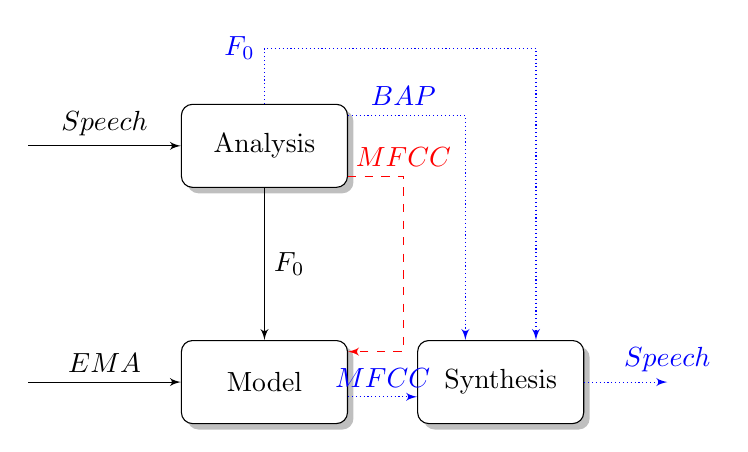
\begin{tikzpicture}[auto, node distance=3cm,>=latex']
    \node [input, name=speech] {};
    
    \node [block, right of=speech] (analysis) {Analysis};
    \node [block, below of=analysis] (model) {Model};
    \node [block, right of=model] (synthesis) {Synthesis};
    \node [input, name=ema, left of=model] {};
    \node [right of=analysis, name=bela] {};
    \draw [->] (speech) -- node {$\text{Speech}$} (analysis);
    \draw [->,color=blue,densely dotted] (model.350) -- node {$\text{MFCC}$} (synthesis.190);
    \draw[->,color=red,dashed] (analysis.340) -- +(2em, 0) node[above] {$\text{MFCC}$} |- (model.380);
    \draw[->] (analysis.270) -- node {$F_0$} (model.90);
    \draw[->,color=blue,densely dotted] (analysis.380) -- +(2em,0) node[above] {$\text{BAP}$} -| (synthesis.130);
    \draw[->,color=blue,densely dotted] (synthesis.0) -- +(3em,0) node[above] {$\text{Speech}$};
    \draw[->] (ema) -- node[above] {$\text{EMA}$} (model);
    \draw[->,color=blue,densely dotted] (analysis.90) -- +(0,2em) node[left] {$F_0$} -| (synthesis.50);
    \end{tikzpicture}
\end{figure}

\begin{table}[th]
  \caption{Comparison of preprocessing techniques}
  \label{tab:example}
  \centering
  \footnotesize
  \begin{tabular}{ r r r r }
    \toprule
    \textbf{Author} & \textbf{Liu} & \textbf{Taguchi} & \textbf{Gonzalez} \\
    \midrule
    \textbf{EMA/PMA} & EMA & EMA & PMA \\
    \textbf{MFCC} & 40 + 1 & 40 + 1 & 24 + 1 \\
    \textbf{Delta} & No & Yes & Yes \\
    \textbf{EMA sampling} & 200 Hz & 200 Hz & 100 Hz* \\
    \textbf{Standardisation} & Yes & Yes & Yes \\
    \textbf{Smoothing} & No & Yes  & No \\
    \textbf{Vocoder} & STRAIGHT \cite{Kawahara2006} & WORLD  & STRAIGHT \\
    \bottomrule
  \end{tabular}
  *upsampled to 200 Hz to match analysis rate
\end{table}

\subsection{Neural network design} \label{section:nnexperiment}

\subsubsection{An empirical look at previous architectures}

In this paper, a recurrent neural network will be used in order to
approximate the articulatory to acoustic mapping. To construct
this speaker-independent network, previous speaker-dependent architectures
have been studied, to conclude on an appropriate design.

It has been concluded that the optimisation schedules of the publications
studied were very different, most likely due to the problem of vanishing and
exploding gradients in recurrent neural networks.
This is the reason why \cite{Taguchi} used incremental
training along with gradient clipping, and probably the reason why \cite{Liu2018} used a learning rate
scheduler. However, \cite{Gonzalez2017} used Adam optimiser \cite{Kingma2015}
which is known to manage both of these problems with the minor disadvantage of
the abscence of good convergence guarantees. The fact that Adam was able
to obtain similar results without careful parameter-tuning indicated that
it will be an appropriate candidate as an optimiser for our model. 

Previous publications on speaker-dependent models reported best
performance on bidirectional architectures, however it was unclear whether
BLSTM or BGRU architectures are better. Also, \cite{Taguchi} resorted to
a combination of fully connected and recurrent layers.

In order to determine the best architecture, a pilot study has been
performed on all three neural networks which are summarised in Table \ref{tab:architectures},
however all of them were trained with an Adam optimiser for the reasons above, and a learning rate
of \( 0.003 \), and a batch size of 100 without noise on MNGU0 dataset.
The best performing neural network was then trained on the entire dataset.

\begin{table}[th]
  \caption{Performance of speaker-independent articulatory to acoustic neural network for 10-fold cross-validation with 95 \% confidence intervals. In the TORGO dataset, different recording sessions were
    kept in different datasets. }
  \label{tab:all_data}
  \centering
  \footnotesize

  \begin{tabular}{ r r r }
    \toprule
    \textbf{Dataset} & Multi-speaker & Single-speaker \\
    & MCD & MCD \\
    \midrule 
    \textbf{Combined result} & 5.31 $\pm$ 0.09 dB & N/A \\  
    \midrule
    \textbf{MNGU0} & 5.93 $\pm$ 0.31 dB & 4.77 dB \\
    \textbf{Female MOCHA-TIMIT} & \textbf{5.02} $\pm$ 0.06 dB  & 5.23 dB \\
    \textbf{Male MOCHA-TIMIT} & \textbf{4.06} $\pm$ 0.06 dB & 5.83 dB \\
    \textbf{TORGO Female 1} & 4.48 $\pm$ 0.03 dB & N/A \\
    \textbf{TORGO Female 2A} & 4.23 $\pm$ 0.06 dB & N/A \\
    \textbf{TORGO Female 2B} & 4.81 $\pm$ 0.14 dB & N/A \\
    \textbf{TORGO Female 3} & 4.94 $\pm$ 0.09 dB & N/A \\
    \textbf{TORGO Male 1A} & 4.64 $\pm$ 0.04 dB & N/A \\
    \textbf{TORGO Male 1B} & 4.70 $\pm$ 0.05 dB & N/A \\
    \textbf{TORGO Male 2A} & 4.62 $\pm$ 0.04 dB & N/A \\
    \textbf{TORGO Male 2B} & 15 $\pm$ 0.86 dB & N/A\\
    \textbf{TORGO Male 3} & 4.63 $\pm$ 0.11 dB & N/A \\
    \textbf{TORGO Male 4} & 4.85 $\pm$ 0.12 dB & N/A \\
    \bottomrule
  \end{tabular}
\end{table}


%\begin{table}[th]
%  \caption{Transfer learning comparison with single speaker models}
%  \label{tab:transfer}
%  \centering
%  \footnotesize
%
%  \begin{tabular}{ r r r}
%    \toprule
%    \textbf{Dataset} & \textbf{Speaker only} & \textbf{Transfer preproc} \\
%    \midrule
%    \textbf{MNGU0} & 4.77 dB & N/A \\
%    \textbf{Female MOCHA-TIMIT} & 5.23 dB & 11.43 dB \\
%    \textbf{Male MOCHA-TIMIT} & 5.88 dB & 7.86 dB \\
%    \bottomrule
%  \end{tabular}
%\end{table}

\begin{table}[th]
  \caption{Comparison of different training methods used in previous publications with the
    results of the pilot study using held-out validation. The method described in the paper of
  Gonzalez performed best.}
  \label{tab:architectures}
  \centering
  \footnotesize

  \begin{tabular}{ r r r r }
    \toprule
    \textbf{Author} & \textbf{Liu} & \textbf{Taguchi} & \textbf{Gonzalez} \\
    \midrule
    \textbf{BLSTM layers} & 4 (128) & 2 (256) & 4 (150) GRU \\
    \textbf{Dense layers} & 1 & 3+1 & 1 \\
    \textbf{Regularisation} & No & LayerNorm & Noise 0.05 \\
    \textbf{Dropout} & No & Yes (50 \%) & No \\
    \textbf{Optimiser} & SGD & RMSProp & Adam \\
    \textbf{Learning rate} & 0.01* & 0.01 & 0.003 \\
    \textbf{Gradient clipping} & No & 5 & No \\
    \textbf{Early stopping} & Yes & Yes & Yes \\
    \textbf{MLPG} \cite{Wu2016} & No & Yes & Yes \\ 
    \textbf{Maximum epochs} & 32 & N/A & 100 \\
    \textbf{Batch size} & N/A & 8 & 100 \\
    \textbf{Incremental training} & No & Yes & Yes \\
    \textbf{MCD***} & 4.84 dB & 7.28 dB & 4.77 dB \\
    \bottomrule
  \end{tabular}
  * with decay after Epoch 11 \\
  ** from author communication \\
  *** results of our training with Adam optimiser
\end{table}

For training the mean squared error loss function was used, and for
evaluation the Mel cepstral distortion (MCD) have been employed. \cite{Kubichek1993}

For the speaker-independent experiments, ten fold cross-validation was performed
to estimate the out-ouf-sample generalisation capability of the neural networks.

\subsection{Articulatory space modification} \label{section:speech}

Using this framework, the problem of making pathological speech
can be traded for the problem of making pathological articulation and
feeding pathological articulation through the neural network.

In order to make the articulation pathological, two methods were employed.
The first method fixes the position of the tongue tip in the initial position.
The second method decreases the velocity of the tongue via thresholding discrete time differences,
and reconstructing the position with performing a cumulative sum.




\section{Results and discussion}

\subsection{Pilot study}

The pilot study results are summarised in Table \ref{tab:example}.

Based on our training, it seems clear that the GRU architecture was superior to an LSTM
architecture in our case, when used with an Adam optimiser.
There is no general consesus whether GRU or LSTM is better for particular
datasets. \cite{Jozefowicz2015}

\subsection{Prediction of MFCC values}

The prediction results for the MFCC values are summarised in Table
\ref{tab:all_data}. Results were all in similar range as previously
reported values for speaker-dependent datasets, and in our framework
the speaker-independent architectures clearly performed better than the
speaker-dependent architectures on the MOCHA-TIMIT datasets.

\subsection{What do these neural networks learn?} \label{section:visualisation}

Recently, there have been many advancements in understanding what neural networks learn.
Convolutional neural networks can be analysed via conventional methods in filter analysis \cite{Palaz2015},
classification neural networks can propagate back gradients to find the most important inputs for
the prediction \cite{Selvaraju2017}. These techniques are not applicable for recurrent neural networks in a regression
context, so we resort to exploring the activations outputs of the layers.

To make these intelligible, a Prewitt mask is thresholded to find peaks in the activations.
On Figure \ref{fig:mask}, two things can be observed. Firstly, line-like boundaries are learned, and their duration indicates these might approximate phone to word level representations. Secondly, as the activations propagate through the deeper layers of the neural networks, these line like boundaries are better approximated.

\subsection{The current limitations of the synthesis} \label{section:limitations}
The quality of the synthetised speech depends on the quality of vocoding and
the quality of prediction.

According to our observations, the quality is bounded more by the
quality of the vocoder, than the synthesis itself. It has been found that mean squared error (MSE) between the vocoder resynthesised speech and the predicted speech is 11 on the MNGU0 dataset. The MSE between the analysis-resynthesis and the vocoder is 80. That means that 88\% of the performance loss
is due to the vocoder analysis-resynthesis. This indicates that
future improvements should focus on better vocoding rather than better
acoustic mapping.

Despite that, we wanted to investigate the sensitivity of the model performance to more
training data. The neural network was retrained using incrementally more training data in twenty
percent batches. The MSE was calculated at all epochs of training for the validation set, which
can be seen on Figure \ref{learning_curve}.

\begin{figure}[t]
  \begin{center}
    \scalebox{0.50}{%% Creator: Matplotlib, PGF backend
%%
%% To include the figure in your LaTeX document, write
%%   \input{<filename>.pgf}
%%
%% Make sure the required packages are loaded in your preamble
%%   \usepackage{pgf}
%%
%% Figures using additional raster images can only be included by \input if
%% they are in the same directory as the main LaTeX file. For loading figures
%% from other directories you can use the `import` package
%%   \usepackage{import}
%% and then include the figures with
%%   \import{<path to file>}{<filename>.pgf}
%%
%% Matplotlib used the following preamble
%%   \usepackage{fontspec}
%%   \setmainfont{DejaVu Serif}
%%   \setsansfont{DejaVu Sans}
%%   \setmonofont{DejaVu Sans Mono}
%%
\begingroup%
\makeatletter%
\begin{pgfpicture}%
\pgfpathrectangle{\pgfpointorigin}{\pgfqpoint{6.400000in}{4.800000in}}%
\pgfusepath{use as bounding box, clip}%
\begin{pgfscope}%
\pgfsetbuttcap%
\pgfsetmiterjoin%
\definecolor{currentfill}{rgb}{1.000000,1.000000,1.000000}%
\pgfsetfillcolor{currentfill}%
\pgfsetlinewidth{0.000000pt}%
\definecolor{currentstroke}{rgb}{1.000000,1.000000,1.000000}%
\pgfsetstrokecolor{currentstroke}%
\pgfsetdash{}{0pt}%
\pgfpathmoveto{\pgfqpoint{0.000000in}{0.000000in}}%
\pgfpathlineto{\pgfqpoint{6.400000in}{0.000000in}}%
\pgfpathlineto{\pgfqpoint{6.400000in}{4.800000in}}%
\pgfpathlineto{\pgfqpoint{0.000000in}{4.800000in}}%
\pgfpathclose%
\pgfusepath{fill}%
\end{pgfscope}%
\begin{pgfscope}%
\pgfsetbuttcap%
\pgfsetmiterjoin%
\definecolor{currentfill}{rgb}{1.000000,1.000000,1.000000}%
\pgfsetfillcolor{currentfill}%
\pgfsetlinewidth{0.000000pt}%
\definecolor{currentstroke}{rgb}{0.000000,0.000000,0.000000}%
\pgfsetstrokecolor{currentstroke}%
\pgfsetstrokeopacity{0.000000}%
\pgfsetdash{}{0pt}%
\pgfpathmoveto{\pgfqpoint{0.800000in}{0.528000in}}%
\pgfpathlineto{\pgfqpoint{5.760000in}{0.528000in}}%
\pgfpathlineto{\pgfqpoint{5.760000in}{4.224000in}}%
\pgfpathlineto{\pgfqpoint{0.800000in}{4.224000in}}%
\pgfpathclose%
\pgfusepath{fill}%
\end{pgfscope}%
\begin{pgfscope}%
\pgfsetbuttcap%
\pgfsetroundjoin%
\definecolor{currentfill}{rgb}{0.000000,0.000000,0.000000}%
\pgfsetfillcolor{currentfill}%
\pgfsetlinewidth{0.803000pt}%
\definecolor{currentstroke}{rgb}{0.000000,0.000000,0.000000}%
\pgfsetstrokecolor{currentstroke}%
\pgfsetdash{}{0pt}%
\pgfsys@defobject{currentmarker}{\pgfqpoint{0.000000in}{-0.048611in}}{\pgfqpoint{0.000000in}{0.000000in}}{%
\pgfpathmoveto{\pgfqpoint{0.000000in}{0.000000in}}%
\pgfpathlineto{\pgfqpoint{0.000000in}{-0.048611in}}%
\pgfusepath{stroke,fill}%
}%
\begin{pgfscope}%
\pgfsys@transformshift{1.025455in}{0.528000in}%
\pgfsys@useobject{currentmarker}{}%
\end{pgfscope}%
\end{pgfscope}%
\begin{pgfscope}%
\pgftext[x=1.025455in,y=0.430778in,,top]{\sffamily\fontsize{10.000000}{12.000000}\selectfont 0}%
\end{pgfscope}%
\begin{pgfscope}%
\pgfsetbuttcap%
\pgfsetroundjoin%
\definecolor{currentfill}{rgb}{0.000000,0.000000,0.000000}%
\pgfsetfillcolor{currentfill}%
\pgfsetlinewidth{0.803000pt}%
\definecolor{currentstroke}{rgb}{0.000000,0.000000,0.000000}%
\pgfsetstrokecolor{currentstroke}%
\pgfsetdash{}{0pt}%
\pgfsys@defobject{currentmarker}{\pgfqpoint{0.000000in}{-0.048611in}}{\pgfqpoint{0.000000in}{0.000000in}}{%
\pgfpathmoveto{\pgfqpoint{0.000000in}{0.000000in}}%
\pgfpathlineto{\pgfqpoint{0.000000in}{-0.048611in}}%
\pgfusepath{stroke,fill}%
}%
\begin{pgfscope}%
\pgfsys@transformshift{1.936382in}{0.528000in}%
\pgfsys@useobject{currentmarker}{}%
\end{pgfscope}%
\end{pgfscope}%
\begin{pgfscope}%
\pgftext[x=1.936382in,y=0.430778in,,top]{\sffamily\fontsize{10.000000}{12.000000}\selectfont 20}%
\end{pgfscope}%
\begin{pgfscope}%
\pgfsetbuttcap%
\pgfsetroundjoin%
\definecolor{currentfill}{rgb}{0.000000,0.000000,0.000000}%
\pgfsetfillcolor{currentfill}%
\pgfsetlinewidth{0.803000pt}%
\definecolor{currentstroke}{rgb}{0.000000,0.000000,0.000000}%
\pgfsetstrokecolor{currentstroke}%
\pgfsetdash{}{0pt}%
\pgfsys@defobject{currentmarker}{\pgfqpoint{0.000000in}{-0.048611in}}{\pgfqpoint{0.000000in}{0.000000in}}{%
\pgfpathmoveto{\pgfqpoint{0.000000in}{0.000000in}}%
\pgfpathlineto{\pgfqpoint{0.000000in}{-0.048611in}}%
\pgfusepath{stroke,fill}%
}%
\begin{pgfscope}%
\pgfsys@transformshift{2.847309in}{0.528000in}%
\pgfsys@useobject{currentmarker}{}%
\end{pgfscope}%
\end{pgfscope}%
\begin{pgfscope}%
\pgftext[x=2.847309in,y=0.430778in,,top]{\sffamily\fontsize{10.000000}{12.000000}\selectfont 40}%
\end{pgfscope}%
\begin{pgfscope}%
\pgfsetbuttcap%
\pgfsetroundjoin%
\definecolor{currentfill}{rgb}{0.000000,0.000000,0.000000}%
\pgfsetfillcolor{currentfill}%
\pgfsetlinewidth{0.803000pt}%
\definecolor{currentstroke}{rgb}{0.000000,0.000000,0.000000}%
\pgfsetstrokecolor{currentstroke}%
\pgfsetdash{}{0pt}%
\pgfsys@defobject{currentmarker}{\pgfqpoint{0.000000in}{-0.048611in}}{\pgfqpoint{0.000000in}{0.000000in}}{%
\pgfpathmoveto{\pgfqpoint{0.000000in}{0.000000in}}%
\pgfpathlineto{\pgfqpoint{0.000000in}{-0.048611in}}%
\pgfusepath{stroke,fill}%
}%
\begin{pgfscope}%
\pgfsys@transformshift{3.758237in}{0.528000in}%
\pgfsys@useobject{currentmarker}{}%
\end{pgfscope}%
\end{pgfscope}%
\begin{pgfscope}%
\pgftext[x=3.758237in,y=0.430778in,,top]{\sffamily\fontsize{10.000000}{12.000000}\selectfont 60}%
\end{pgfscope}%
\begin{pgfscope}%
\pgfsetbuttcap%
\pgfsetroundjoin%
\definecolor{currentfill}{rgb}{0.000000,0.000000,0.000000}%
\pgfsetfillcolor{currentfill}%
\pgfsetlinewidth{0.803000pt}%
\definecolor{currentstroke}{rgb}{0.000000,0.000000,0.000000}%
\pgfsetstrokecolor{currentstroke}%
\pgfsetdash{}{0pt}%
\pgfsys@defobject{currentmarker}{\pgfqpoint{0.000000in}{-0.048611in}}{\pgfqpoint{0.000000in}{0.000000in}}{%
\pgfpathmoveto{\pgfqpoint{0.000000in}{0.000000in}}%
\pgfpathlineto{\pgfqpoint{0.000000in}{-0.048611in}}%
\pgfusepath{stroke,fill}%
}%
\begin{pgfscope}%
\pgfsys@transformshift{4.669164in}{0.528000in}%
\pgfsys@useobject{currentmarker}{}%
\end{pgfscope}%
\end{pgfscope}%
\begin{pgfscope}%
\pgftext[x=4.669164in,y=0.430778in,,top]{\sffamily\fontsize{10.000000}{12.000000}\selectfont 80}%
\end{pgfscope}%
\begin{pgfscope}%
\pgfsetbuttcap%
\pgfsetroundjoin%
\definecolor{currentfill}{rgb}{0.000000,0.000000,0.000000}%
\pgfsetfillcolor{currentfill}%
\pgfsetlinewidth{0.803000pt}%
\definecolor{currentstroke}{rgb}{0.000000,0.000000,0.000000}%
\pgfsetstrokecolor{currentstroke}%
\pgfsetdash{}{0pt}%
\pgfsys@defobject{currentmarker}{\pgfqpoint{0.000000in}{-0.048611in}}{\pgfqpoint{0.000000in}{0.000000in}}{%
\pgfpathmoveto{\pgfqpoint{0.000000in}{0.000000in}}%
\pgfpathlineto{\pgfqpoint{0.000000in}{-0.048611in}}%
\pgfusepath{stroke,fill}%
}%
\begin{pgfscope}%
\pgfsys@transformshift{5.580092in}{0.528000in}%
\pgfsys@useobject{currentmarker}{}%
\end{pgfscope}%
\end{pgfscope}%
\begin{pgfscope}%
\pgftext[x=5.580092in,y=0.430778in,,top]{\sffamily\fontsize{10.000000}{12.000000}\selectfont 100}%
\end{pgfscope}%
\begin{pgfscope}%
\pgftext[x=3.280000in,y=0.240809in,,top]{\sffamily\fontsize{10.000000}{12.000000}\selectfont Epochs}%
\end{pgfscope}%
\begin{pgfscope}%
\pgfsetbuttcap%
\pgfsetroundjoin%
\definecolor{currentfill}{rgb}{0.000000,0.000000,0.000000}%
\pgfsetfillcolor{currentfill}%
\pgfsetlinewidth{0.803000pt}%
\definecolor{currentstroke}{rgb}{0.000000,0.000000,0.000000}%
\pgfsetstrokecolor{currentstroke}%
\pgfsetdash{}{0pt}%
\pgfsys@defobject{currentmarker}{\pgfqpoint{-0.048611in}{0.000000in}}{\pgfqpoint{0.000000in}{0.000000in}}{%
\pgfpathmoveto{\pgfqpoint{0.000000in}{0.000000in}}%
\pgfpathlineto{\pgfqpoint{-0.048611in}{0.000000in}}%
\pgfusepath{stroke,fill}%
}%
\begin{pgfscope}%
\pgfsys@transformshift{0.800000in}{0.921416in}%
\pgfsys@useobject{currentmarker}{}%
\end{pgfscope}%
\end{pgfscope}%
\begin{pgfscope}%
\pgftext[x=0.393533in,y=0.868654in,left,base]{\sffamily\fontsize{10.000000}{12.000000}\selectfont 0.50}%
\end{pgfscope}%
\begin{pgfscope}%
\pgfsetbuttcap%
\pgfsetroundjoin%
\definecolor{currentfill}{rgb}{0.000000,0.000000,0.000000}%
\pgfsetfillcolor{currentfill}%
\pgfsetlinewidth{0.803000pt}%
\definecolor{currentstroke}{rgb}{0.000000,0.000000,0.000000}%
\pgfsetstrokecolor{currentstroke}%
\pgfsetdash{}{0pt}%
\pgfsys@defobject{currentmarker}{\pgfqpoint{-0.048611in}{0.000000in}}{\pgfqpoint{0.000000in}{0.000000in}}{%
\pgfpathmoveto{\pgfqpoint{0.000000in}{0.000000in}}%
\pgfpathlineto{\pgfqpoint{-0.048611in}{0.000000in}}%
\pgfusepath{stroke,fill}%
}%
\begin{pgfscope}%
\pgfsys@transformshift{0.800000in}{1.621655in}%
\pgfsys@useobject{currentmarker}{}%
\end{pgfscope}%
\end{pgfscope}%
\begin{pgfscope}%
\pgftext[x=0.393533in,y=1.568893in,left,base]{\sffamily\fontsize{10.000000}{12.000000}\selectfont 0.55}%
\end{pgfscope}%
\begin{pgfscope}%
\pgfsetbuttcap%
\pgfsetroundjoin%
\definecolor{currentfill}{rgb}{0.000000,0.000000,0.000000}%
\pgfsetfillcolor{currentfill}%
\pgfsetlinewidth{0.803000pt}%
\definecolor{currentstroke}{rgb}{0.000000,0.000000,0.000000}%
\pgfsetstrokecolor{currentstroke}%
\pgfsetdash{}{0pt}%
\pgfsys@defobject{currentmarker}{\pgfqpoint{-0.048611in}{0.000000in}}{\pgfqpoint{0.000000in}{0.000000in}}{%
\pgfpathmoveto{\pgfqpoint{0.000000in}{0.000000in}}%
\pgfpathlineto{\pgfqpoint{-0.048611in}{0.000000in}}%
\pgfusepath{stroke,fill}%
}%
\begin{pgfscope}%
\pgfsys@transformshift{0.800000in}{2.321894in}%
\pgfsys@useobject{currentmarker}{}%
\end{pgfscope}%
\end{pgfscope}%
\begin{pgfscope}%
\pgftext[x=0.393533in,y=2.269133in,left,base]{\sffamily\fontsize{10.000000}{12.000000}\selectfont 0.60}%
\end{pgfscope}%
\begin{pgfscope}%
\pgfsetbuttcap%
\pgfsetroundjoin%
\definecolor{currentfill}{rgb}{0.000000,0.000000,0.000000}%
\pgfsetfillcolor{currentfill}%
\pgfsetlinewidth{0.803000pt}%
\definecolor{currentstroke}{rgb}{0.000000,0.000000,0.000000}%
\pgfsetstrokecolor{currentstroke}%
\pgfsetdash{}{0pt}%
\pgfsys@defobject{currentmarker}{\pgfqpoint{-0.048611in}{0.000000in}}{\pgfqpoint{0.000000in}{0.000000in}}{%
\pgfpathmoveto{\pgfqpoint{0.000000in}{0.000000in}}%
\pgfpathlineto{\pgfqpoint{-0.048611in}{0.000000in}}%
\pgfusepath{stroke,fill}%
}%
\begin{pgfscope}%
\pgfsys@transformshift{0.800000in}{3.022134in}%
\pgfsys@useobject{currentmarker}{}%
\end{pgfscope}%
\end{pgfscope}%
\begin{pgfscope}%
\pgftext[x=0.393533in,y=2.969372in,left,base]{\sffamily\fontsize{10.000000}{12.000000}\selectfont 0.65}%
\end{pgfscope}%
\begin{pgfscope}%
\pgfsetbuttcap%
\pgfsetroundjoin%
\definecolor{currentfill}{rgb}{0.000000,0.000000,0.000000}%
\pgfsetfillcolor{currentfill}%
\pgfsetlinewidth{0.803000pt}%
\definecolor{currentstroke}{rgb}{0.000000,0.000000,0.000000}%
\pgfsetstrokecolor{currentstroke}%
\pgfsetdash{}{0pt}%
\pgfsys@defobject{currentmarker}{\pgfqpoint{-0.048611in}{0.000000in}}{\pgfqpoint{0.000000in}{0.000000in}}{%
\pgfpathmoveto{\pgfqpoint{0.000000in}{0.000000in}}%
\pgfpathlineto{\pgfqpoint{-0.048611in}{0.000000in}}%
\pgfusepath{stroke,fill}%
}%
\begin{pgfscope}%
\pgfsys@transformshift{0.800000in}{3.722373in}%
\pgfsys@useobject{currentmarker}{}%
\end{pgfscope}%
\end{pgfscope}%
\begin{pgfscope}%
\pgftext[x=0.393533in,y=3.669611in,left,base]{\sffamily\fontsize{10.000000}{12.000000}\selectfont 0.70}%
\end{pgfscope}%
\begin{pgfscope}%
\pgftext[x=0.337977in,y=2.376000in,,bottom,rotate=90.000000]{\sffamily\fontsize{10.000000}{12.000000}\selectfont Validation loss}%
\end{pgfscope}%
\begin{pgfscope}%
\pgfpathrectangle{\pgfqpoint{0.800000in}{0.528000in}}{\pgfqpoint{4.960000in}{3.696000in}}%
\pgfusepath{clip}%
\pgfsetrectcap%
\pgfsetroundjoin%
\pgfsetlinewidth{1.505625pt}%
\definecolor{currentstroke}{rgb}{0.121569,0.466667,0.705882}%
\pgfsetstrokecolor{currentstroke}%
\pgfsetdash{}{0pt}%
\pgfpathmoveto{\pgfqpoint{1.025455in}{3.329852in}}%
\pgfpathlineto{\pgfqpoint{1.071001in}{2.411908in}}%
\pgfpathlineto{\pgfqpoint{1.116547in}{2.257215in}}%
\pgfpathlineto{\pgfqpoint{1.162094in}{1.847696in}}%
\pgfpathlineto{\pgfqpoint{1.207640in}{1.873978in}}%
\pgfpathlineto{\pgfqpoint{1.253186in}{1.503324in}}%
\pgfpathlineto{\pgfqpoint{1.298733in}{1.449766in}}%
\pgfpathlineto{\pgfqpoint{1.344279in}{1.293240in}}%
\pgfpathlineto{\pgfqpoint{1.389826in}{1.197630in}}%
\pgfpathlineto{\pgfqpoint{1.435372in}{1.101648in}}%
\pgfpathlineto{\pgfqpoint{1.480918in}{1.058666in}}%
\pgfpathlineto{\pgfqpoint{1.526465in}{1.047333in}}%
\pgfpathlineto{\pgfqpoint{1.572011in}{0.899145in}}%
\pgfpathlineto{\pgfqpoint{1.617557in}{0.894948in}}%
\pgfpathlineto{\pgfqpoint{1.663104in}{0.850535in}}%
\pgfpathlineto{\pgfqpoint{1.708650in}{0.835844in}}%
\pgfpathlineto{\pgfqpoint{1.754197in}{0.908905in}}%
\pgfpathlineto{\pgfqpoint{1.799743in}{0.845967in}}%
\pgfpathlineto{\pgfqpoint{1.845289in}{0.831257in}}%
\pgfpathlineto{\pgfqpoint{1.890836in}{0.816295in}}%
\pgfpathlineto{\pgfqpoint{1.936382in}{0.696000in}}%
\pgfpathlineto{\pgfqpoint{1.981928in}{0.852622in}}%
\pgfpathlineto{\pgfqpoint{2.027475in}{0.886335in}}%
\pgfpathlineto{\pgfqpoint{2.073021in}{0.750419in}}%
\pgfpathlineto{\pgfqpoint{2.118567in}{0.818833in}}%
\pgfpathlineto{\pgfqpoint{2.164114in}{0.750885in}}%
\pgfpathlineto{\pgfqpoint{2.209660in}{0.878928in}}%
\pgfpathlineto{\pgfqpoint{2.255207in}{0.864616in}}%
\pgfpathlineto{\pgfqpoint{2.300753in}{0.897478in}}%
\pgfpathlineto{\pgfqpoint{2.346299in}{0.911367in}}%
\pgfpathlineto{\pgfqpoint{2.391846in}{0.948280in}}%
\pgfpathlineto{\pgfqpoint{2.437392in}{0.852626in}}%
\pgfpathlineto{\pgfqpoint{2.482938in}{0.990058in}}%
\pgfpathlineto{\pgfqpoint{2.528485in}{0.831758in}}%
\pgfpathlineto{\pgfqpoint{2.574031in}{0.940458in}}%
\pgfpathlineto{\pgfqpoint{2.619578in}{0.921133in}}%
\pgfpathlineto{\pgfqpoint{2.665124in}{0.867181in}}%
\pgfpathlineto{\pgfqpoint{2.710670in}{0.981688in}}%
\pgfpathlineto{\pgfqpoint{2.756217in}{0.703079in}}%
\pgfpathlineto{\pgfqpoint{2.801763in}{0.906677in}}%
\pgfpathlineto{\pgfqpoint{2.847309in}{0.915519in}}%
\pgfpathlineto{\pgfqpoint{2.892856in}{1.018872in}}%
\pgfpathlineto{\pgfqpoint{2.938402in}{0.944290in}}%
\pgfpathlineto{\pgfqpoint{2.983949in}{0.863761in}}%
\pgfpathlineto{\pgfqpoint{3.029495in}{1.070475in}}%
\pgfpathlineto{\pgfqpoint{3.075041in}{0.943493in}}%
\pgfpathlineto{\pgfqpoint{3.120588in}{1.073580in}}%
\pgfpathlineto{\pgfqpoint{3.166134in}{1.002707in}}%
\pgfpathlineto{\pgfqpoint{3.211680in}{1.009071in}}%
\pgfpathlineto{\pgfqpoint{3.257227in}{1.114837in}}%
\pgfpathlineto{\pgfqpoint{3.302773in}{0.947863in}}%
\pgfpathlineto{\pgfqpoint{3.348320in}{1.009451in}}%
\pgfpathlineto{\pgfqpoint{3.393866in}{1.103222in}}%
\pgfpathlineto{\pgfqpoint{3.439412in}{1.009327in}}%
\pgfpathlineto{\pgfqpoint{3.484959in}{1.160038in}}%
\pgfpathlineto{\pgfqpoint{3.530505in}{1.106916in}}%
\pgfpathlineto{\pgfqpoint{3.576051in}{1.160081in}}%
\pgfpathlineto{\pgfqpoint{3.621598in}{1.080460in}}%
\pgfpathlineto{\pgfqpoint{3.667144in}{1.069993in}}%
\pgfpathlineto{\pgfqpoint{3.712691in}{1.132873in}}%
\pgfpathlineto{\pgfqpoint{3.758237in}{1.085410in}}%
\pgfpathlineto{\pgfqpoint{3.803783in}{0.985480in}}%
\pgfpathlineto{\pgfqpoint{3.849330in}{1.104155in}}%
\pgfpathlineto{\pgfqpoint{3.894876in}{1.078982in}}%
\pgfpathlineto{\pgfqpoint{3.940422in}{0.974199in}}%
\pgfpathlineto{\pgfqpoint{3.985969in}{1.051528in}}%
\pgfpathlineto{\pgfqpoint{4.031515in}{1.216164in}}%
\pgfpathlineto{\pgfqpoint{4.077062in}{1.081358in}}%
\pgfpathlineto{\pgfqpoint{4.122608in}{1.059803in}}%
\pgfpathlineto{\pgfqpoint{4.168154in}{1.151726in}}%
\pgfpathlineto{\pgfqpoint{4.213701in}{1.113120in}}%
\pgfpathlineto{\pgfqpoint{4.259247in}{1.094570in}}%
\pgfpathlineto{\pgfqpoint{4.304793in}{1.185883in}}%
\pgfpathlineto{\pgfqpoint{4.350340in}{1.053668in}}%
\pgfpathlineto{\pgfqpoint{4.395886in}{1.181144in}}%
\pgfpathlineto{\pgfqpoint{4.441433in}{1.049968in}}%
\pgfpathlineto{\pgfqpoint{4.486979in}{1.069337in}}%
\pgfpathlineto{\pgfqpoint{4.532525in}{1.182916in}}%
\pgfpathlineto{\pgfqpoint{4.578072in}{1.250479in}}%
\pgfpathlineto{\pgfqpoint{4.623618in}{2.492374in}}%
\pgfpathlineto{\pgfqpoint{4.669164in}{1.377734in}}%
\pgfpathlineto{\pgfqpoint{4.714711in}{1.198487in}}%
\pgfpathlineto{\pgfqpoint{4.760257in}{1.087646in}}%
\pgfpathlineto{\pgfqpoint{4.805803in}{0.942623in}}%
\pgfpathlineto{\pgfqpoint{4.851350in}{0.860352in}}%
\pgfpathlineto{\pgfqpoint{4.896896in}{1.009840in}}%
\pgfpathlineto{\pgfqpoint{4.942443in}{0.917959in}}%
\pgfpathlineto{\pgfqpoint{4.987989in}{0.982708in}}%
\pgfpathlineto{\pgfqpoint{5.033535in}{0.907599in}}%
\pgfpathlineto{\pgfqpoint{5.079082in}{0.936577in}}%
\pgfpathlineto{\pgfqpoint{5.124628in}{1.015665in}}%
\pgfpathlineto{\pgfqpoint{5.170174in}{0.964665in}}%
\pgfpathlineto{\pgfqpoint{5.215721in}{1.047464in}}%
\pgfpathlineto{\pgfqpoint{5.261267in}{1.083462in}}%
\pgfpathlineto{\pgfqpoint{5.306814in}{0.990945in}}%
\pgfpathlineto{\pgfqpoint{5.352360in}{1.018657in}}%
\pgfpathlineto{\pgfqpoint{5.397906in}{1.030744in}}%
\pgfpathlineto{\pgfqpoint{5.443453in}{1.022988in}}%
\pgfpathlineto{\pgfqpoint{5.488999in}{1.007689in}}%
\pgfpathlineto{\pgfqpoint{5.534545in}{1.020802in}}%
\pgfusepath{stroke}%
\end{pgfscope}%
\begin{pgfscope}%
\pgfpathrectangle{\pgfqpoint{0.800000in}{0.528000in}}{\pgfqpoint{4.960000in}{3.696000in}}%
\pgfusepath{clip}%
\pgfsetrectcap%
\pgfsetroundjoin%
\pgfsetlinewidth{1.505625pt}%
\definecolor{currentstroke}{rgb}{1.000000,0.498039,0.054902}%
\pgfsetstrokecolor{currentstroke}%
\pgfsetdash{}{0pt}%
\pgfpathmoveto{\pgfqpoint{1.025455in}{3.497344in}}%
\pgfpathlineto{\pgfqpoint{1.071001in}{2.761286in}}%
\pgfpathlineto{\pgfqpoint{1.116547in}{2.395856in}}%
\pgfpathlineto{\pgfqpoint{1.162094in}{2.269842in}}%
\pgfpathlineto{\pgfqpoint{1.207640in}{1.931499in}}%
\pgfpathlineto{\pgfqpoint{1.253186in}{1.808361in}}%
\pgfpathlineto{\pgfqpoint{1.298733in}{1.808719in}}%
\pgfpathlineto{\pgfqpoint{1.344279in}{1.601188in}}%
\pgfpathlineto{\pgfqpoint{1.389826in}{1.401837in}}%
\pgfpathlineto{\pgfqpoint{1.435372in}{1.275346in}}%
\pgfpathlineto{\pgfqpoint{1.480918in}{1.198450in}}%
\pgfpathlineto{\pgfqpoint{1.526465in}{1.158741in}}%
\pgfpathlineto{\pgfqpoint{1.572011in}{1.156719in}}%
\pgfpathlineto{\pgfqpoint{1.617557in}{0.947966in}}%
\pgfpathlineto{\pgfqpoint{1.663104in}{1.109757in}}%
\pgfpathlineto{\pgfqpoint{1.708650in}{0.968993in}}%
\pgfpathlineto{\pgfqpoint{1.754197in}{0.923454in}}%
\pgfpathlineto{\pgfqpoint{1.799743in}{0.945339in}}%
\pgfpathlineto{\pgfqpoint{1.845289in}{0.917409in}}%
\pgfpathlineto{\pgfqpoint{1.890836in}{0.952825in}}%
\pgfpathlineto{\pgfqpoint{1.936382in}{0.940700in}}%
\pgfpathlineto{\pgfqpoint{1.981928in}{0.914050in}}%
\pgfpathlineto{\pgfqpoint{2.027475in}{0.950115in}}%
\pgfpathlineto{\pgfqpoint{2.073021in}{1.048688in}}%
\pgfpathlineto{\pgfqpoint{2.118567in}{0.961122in}}%
\pgfpathlineto{\pgfqpoint{2.164114in}{0.981333in}}%
\pgfpathlineto{\pgfqpoint{2.209660in}{0.963387in}}%
\pgfpathlineto{\pgfqpoint{2.255207in}{1.047494in}}%
\pgfpathlineto{\pgfqpoint{2.300753in}{0.938878in}}%
\pgfpathlineto{\pgfqpoint{2.346299in}{1.060513in}}%
\pgfpathlineto{\pgfqpoint{2.391846in}{1.097560in}}%
\pgfpathlineto{\pgfqpoint{2.437392in}{1.047835in}}%
\pgfpathlineto{\pgfqpoint{2.482938in}{1.054765in}}%
\pgfpathlineto{\pgfqpoint{2.528485in}{1.068760in}}%
\pgfpathlineto{\pgfqpoint{2.574031in}{1.005912in}}%
\pgfpathlineto{\pgfqpoint{2.619578in}{1.083467in}}%
\pgfpathlineto{\pgfqpoint{2.665124in}{1.003209in}}%
\pgfpathlineto{\pgfqpoint{2.710670in}{1.024399in}}%
\pgfpathlineto{\pgfqpoint{2.756217in}{1.106160in}}%
\pgfpathlineto{\pgfqpoint{2.801763in}{1.078401in}}%
\pgfpathlineto{\pgfqpoint{2.847309in}{1.041596in}}%
\pgfpathlineto{\pgfqpoint{2.892856in}{1.063102in}}%
\pgfpathlineto{\pgfqpoint{2.938402in}{1.217033in}}%
\pgfpathlineto{\pgfqpoint{2.983949in}{1.085574in}}%
\pgfpathlineto{\pgfqpoint{3.029495in}{1.158275in}}%
\pgfpathlineto{\pgfqpoint{3.075041in}{1.162518in}}%
\pgfpathlineto{\pgfqpoint{3.120588in}{1.227529in}}%
\pgfpathlineto{\pgfqpoint{3.166134in}{1.281237in}}%
\pgfpathlineto{\pgfqpoint{3.211680in}{1.301882in}}%
\pgfpathlineto{\pgfqpoint{3.257227in}{1.109609in}}%
\pgfpathlineto{\pgfqpoint{3.302773in}{1.068220in}}%
\pgfpathlineto{\pgfqpoint{3.348320in}{1.053922in}}%
\pgfpathlineto{\pgfqpoint{3.393866in}{1.225248in}}%
\pgfpathlineto{\pgfqpoint{3.439412in}{1.205100in}}%
\pgfpathlineto{\pgfqpoint{3.484959in}{1.188377in}}%
\pgfpathlineto{\pgfqpoint{3.530505in}{1.189022in}}%
\pgfpathlineto{\pgfqpoint{3.576051in}{1.244085in}}%
\pgfpathlineto{\pgfqpoint{3.621598in}{1.214379in}}%
\pgfpathlineto{\pgfqpoint{3.667144in}{1.366302in}}%
\pgfpathlineto{\pgfqpoint{3.712691in}{1.311807in}}%
\pgfpathlineto{\pgfqpoint{3.758237in}{1.274073in}}%
\pgfpathlineto{\pgfqpoint{3.803783in}{1.261234in}}%
\pgfpathlineto{\pgfqpoint{3.849330in}{1.404810in}}%
\pgfpathlineto{\pgfqpoint{3.894876in}{1.297017in}}%
\pgfpathlineto{\pgfqpoint{3.940422in}{1.299920in}}%
\pgfpathlineto{\pgfqpoint{3.985969in}{1.236185in}}%
\pgfpathlineto{\pgfqpoint{4.031515in}{1.415532in}}%
\pgfpathlineto{\pgfqpoint{4.077062in}{1.249183in}}%
\pgfpathlineto{\pgfqpoint{4.122608in}{1.265644in}}%
\pgfpathlineto{\pgfqpoint{4.168154in}{1.351998in}}%
\pgfpathlineto{\pgfqpoint{4.213701in}{1.328812in}}%
\pgfpathlineto{\pgfqpoint{4.259247in}{1.418100in}}%
\pgfpathlineto{\pgfqpoint{4.304793in}{1.388275in}}%
\pgfpathlineto{\pgfqpoint{4.350340in}{1.356505in}}%
\pgfpathlineto{\pgfqpoint{4.395886in}{1.264825in}}%
\pgfpathlineto{\pgfqpoint{4.441433in}{1.373443in}}%
\pgfpathlineto{\pgfqpoint{4.486979in}{1.415896in}}%
\pgfpathlineto{\pgfqpoint{4.532525in}{1.413990in}}%
\pgfpathlineto{\pgfqpoint{4.578072in}{1.447654in}}%
\pgfpathlineto{\pgfqpoint{4.623618in}{1.418146in}}%
\pgfpathlineto{\pgfqpoint{4.669164in}{1.488686in}}%
\pgfpathlineto{\pgfqpoint{4.714711in}{1.454639in}}%
\pgfpathlineto{\pgfqpoint{4.760257in}{1.352422in}}%
\pgfpathlineto{\pgfqpoint{4.805803in}{1.407561in}}%
\pgfpathlineto{\pgfqpoint{4.851350in}{1.432238in}}%
\pgfpathlineto{\pgfqpoint{4.896896in}{1.409070in}}%
\pgfpathlineto{\pgfqpoint{4.942443in}{1.425470in}}%
\pgfpathlineto{\pgfqpoint{4.987989in}{1.505042in}}%
\pgfpathlineto{\pgfqpoint{5.033535in}{1.429005in}}%
\pgfpathlineto{\pgfqpoint{5.079082in}{1.477254in}}%
\pgfpathlineto{\pgfqpoint{5.124628in}{1.491097in}}%
\pgfpathlineto{\pgfqpoint{5.170174in}{1.458299in}}%
\pgfpathlineto{\pgfqpoint{5.215721in}{1.447651in}}%
\pgfpathlineto{\pgfqpoint{5.261267in}{1.352165in}}%
\pgfpathlineto{\pgfqpoint{5.306814in}{1.577379in}}%
\pgfpathlineto{\pgfqpoint{5.352360in}{1.436026in}}%
\pgfpathlineto{\pgfqpoint{5.397906in}{1.341085in}}%
\pgfpathlineto{\pgfqpoint{5.443453in}{1.459381in}}%
\pgfpathlineto{\pgfqpoint{5.488999in}{1.404150in}}%
\pgfpathlineto{\pgfqpoint{5.534545in}{1.523361in}}%
\pgfusepath{stroke}%
\end{pgfscope}%
\begin{pgfscope}%
\pgfpathrectangle{\pgfqpoint{0.800000in}{0.528000in}}{\pgfqpoint{4.960000in}{3.696000in}}%
\pgfusepath{clip}%
\pgfsetrectcap%
\pgfsetroundjoin%
\pgfsetlinewidth{1.505625pt}%
\definecolor{currentstroke}{rgb}{0.172549,0.627451,0.172549}%
\pgfsetstrokecolor{currentstroke}%
\pgfsetdash{}{0pt}%
\pgfpathmoveto{\pgfqpoint{1.025455in}{3.873403in}}%
\pgfpathlineto{\pgfqpoint{1.071001in}{3.242260in}}%
\pgfpathlineto{\pgfqpoint{1.116547in}{2.791029in}}%
\pgfpathlineto{\pgfqpoint{1.162094in}{2.476225in}}%
\pgfpathlineto{\pgfqpoint{1.207640in}{2.342060in}}%
\pgfpathlineto{\pgfqpoint{1.253186in}{2.100891in}}%
\pgfpathlineto{\pgfqpoint{1.298733in}{2.009315in}}%
\pgfpathlineto{\pgfqpoint{1.344279in}{2.021043in}}%
\pgfpathlineto{\pgfqpoint{1.389826in}{1.824885in}}%
\pgfpathlineto{\pgfqpoint{1.435372in}{1.684328in}}%
\pgfpathlineto{\pgfqpoint{1.480918in}{1.745849in}}%
\pgfpathlineto{\pgfqpoint{1.526465in}{1.563984in}}%
\pgfpathlineto{\pgfqpoint{1.572011in}{1.644588in}}%
\pgfpathlineto{\pgfqpoint{1.617557in}{1.575914in}}%
\pgfpathlineto{\pgfqpoint{1.663104in}{1.365875in}}%
\pgfpathlineto{\pgfqpoint{1.708650in}{1.360060in}}%
\pgfpathlineto{\pgfqpoint{1.754197in}{1.211739in}}%
\pgfpathlineto{\pgfqpoint{1.799743in}{1.225226in}}%
\pgfpathlineto{\pgfqpoint{1.845289in}{1.193210in}}%
\pgfpathlineto{\pgfqpoint{1.890836in}{1.090846in}}%
\pgfpathlineto{\pgfqpoint{1.936382in}{1.127688in}}%
\pgfpathlineto{\pgfqpoint{1.981928in}{1.117075in}}%
\pgfpathlineto{\pgfqpoint{2.027475in}{1.192510in}}%
\pgfpathlineto{\pgfqpoint{2.073021in}{1.214926in}}%
\pgfpathlineto{\pgfqpoint{2.118567in}{1.171457in}}%
\pgfpathlineto{\pgfqpoint{2.164114in}{1.110963in}}%
\pgfpathlineto{\pgfqpoint{2.209660in}{1.203423in}}%
\pgfpathlineto{\pgfqpoint{2.255207in}{1.198488in}}%
\pgfpathlineto{\pgfqpoint{2.300753in}{1.141404in}}%
\pgfpathlineto{\pgfqpoint{2.346299in}{1.340845in}}%
\pgfpathlineto{\pgfqpoint{2.391846in}{1.260955in}}%
\pgfpathlineto{\pgfqpoint{2.437392in}{1.295540in}}%
\pgfpathlineto{\pgfqpoint{2.482938in}{1.283076in}}%
\pgfpathlineto{\pgfqpoint{2.528485in}{1.250558in}}%
\pgfpathlineto{\pgfqpoint{2.574031in}{1.339201in}}%
\pgfpathlineto{\pgfqpoint{2.619578in}{1.260238in}}%
\pgfpathlineto{\pgfqpoint{2.665124in}{1.362677in}}%
\pgfpathlineto{\pgfqpoint{2.710670in}{1.312747in}}%
\pgfpathlineto{\pgfqpoint{2.756217in}{1.248516in}}%
\pgfpathlineto{\pgfqpoint{2.801763in}{1.256546in}}%
\pgfpathlineto{\pgfqpoint{2.847309in}{1.430434in}}%
\pgfpathlineto{\pgfqpoint{2.892856in}{1.327699in}}%
\pgfpathlineto{\pgfqpoint{2.938402in}{1.324739in}}%
\pgfpathlineto{\pgfqpoint{2.983949in}{1.485167in}}%
\pgfpathlineto{\pgfqpoint{3.029495in}{1.354856in}}%
\pgfpathlineto{\pgfqpoint{3.075041in}{1.465240in}}%
\pgfpathlineto{\pgfqpoint{3.120588in}{1.325260in}}%
\pgfpathlineto{\pgfqpoint{3.166134in}{1.537541in}}%
\pgfpathlineto{\pgfqpoint{3.211680in}{1.392992in}}%
\pgfpathlineto{\pgfqpoint{3.257227in}{1.505844in}}%
\pgfpathlineto{\pgfqpoint{3.302773in}{1.533912in}}%
\pgfpathlineto{\pgfqpoint{3.348320in}{1.487033in}}%
\pgfpathlineto{\pgfqpoint{3.393866in}{1.438081in}}%
\pgfpathlineto{\pgfqpoint{3.439412in}{1.462604in}}%
\pgfpathlineto{\pgfqpoint{3.484959in}{1.553386in}}%
\pgfpathlineto{\pgfqpoint{3.530505in}{1.674585in}}%
\pgfpathlineto{\pgfqpoint{3.576051in}{1.528382in}}%
\pgfpathlineto{\pgfqpoint{3.621598in}{1.532376in}}%
\pgfpathlineto{\pgfqpoint{3.667144in}{1.660004in}}%
\pgfpathlineto{\pgfqpoint{3.712691in}{1.582824in}}%
\pgfpathlineto{\pgfqpoint{3.758237in}{1.577505in}}%
\pgfpathlineto{\pgfqpoint{3.803783in}{1.539286in}}%
\pgfpathlineto{\pgfqpoint{3.849330in}{1.614645in}}%
\pgfpathlineto{\pgfqpoint{3.894876in}{1.682737in}}%
\pgfpathlineto{\pgfqpoint{3.940422in}{1.696903in}}%
\pgfpathlineto{\pgfqpoint{3.985969in}{1.627033in}}%
\pgfpathlineto{\pgfqpoint{4.031515in}{1.619482in}}%
\pgfpathlineto{\pgfqpoint{4.077062in}{1.610823in}}%
\pgfpathlineto{\pgfqpoint{4.122608in}{1.711002in}}%
\pgfpathlineto{\pgfqpoint{4.168154in}{1.676370in}}%
\pgfpathlineto{\pgfqpoint{4.213701in}{1.744979in}}%
\pgfpathlineto{\pgfqpoint{4.259247in}{1.746352in}}%
\pgfpathlineto{\pgfqpoint{4.304793in}{1.715011in}}%
\pgfpathlineto{\pgfqpoint{4.350340in}{1.700040in}}%
\pgfpathlineto{\pgfqpoint{4.395886in}{1.690854in}}%
\pgfpathlineto{\pgfqpoint{4.441433in}{1.712234in}}%
\pgfpathlineto{\pgfqpoint{4.486979in}{1.691367in}}%
\pgfpathlineto{\pgfqpoint{4.532525in}{1.701754in}}%
\pgfpathlineto{\pgfqpoint{4.578072in}{1.804546in}}%
\pgfpathlineto{\pgfqpoint{4.623618in}{1.715544in}}%
\pgfpathlineto{\pgfqpoint{4.669164in}{1.787755in}}%
\pgfpathlineto{\pgfqpoint{4.714711in}{1.822553in}}%
\pgfpathlineto{\pgfqpoint{4.760257in}{1.789782in}}%
\pgfpathlineto{\pgfqpoint{4.805803in}{1.779803in}}%
\pgfpathlineto{\pgfqpoint{4.851350in}{1.869501in}}%
\pgfpathlineto{\pgfqpoint{4.896896in}{1.781350in}}%
\pgfpathlineto{\pgfqpoint{4.942443in}{1.799178in}}%
\pgfpathlineto{\pgfqpoint{4.987989in}{1.741794in}}%
\pgfpathlineto{\pgfqpoint{5.033535in}{1.778212in}}%
\pgfpathlineto{\pgfqpoint{5.079082in}{1.911867in}}%
\pgfpathlineto{\pgfqpoint{5.124628in}{1.888507in}}%
\pgfpathlineto{\pgfqpoint{5.170174in}{1.940528in}}%
\pgfpathlineto{\pgfqpoint{5.215721in}{1.797561in}}%
\pgfpathlineto{\pgfqpoint{5.261267in}{1.887181in}}%
\pgfpathlineto{\pgfqpoint{5.306814in}{1.782765in}}%
\pgfpathlineto{\pgfqpoint{5.352360in}{1.896270in}}%
\pgfpathlineto{\pgfqpoint{5.397906in}{1.996717in}}%
\pgfpathlineto{\pgfqpoint{5.443453in}{1.971810in}}%
\pgfpathlineto{\pgfqpoint{5.488999in}{1.867460in}}%
\pgfpathlineto{\pgfqpoint{5.534545in}{1.967429in}}%
\pgfusepath{stroke}%
\end{pgfscope}%
\begin{pgfscope}%
\pgfpathrectangle{\pgfqpoint{0.800000in}{0.528000in}}{\pgfqpoint{4.960000in}{3.696000in}}%
\pgfusepath{clip}%
\pgfsetrectcap%
\pgfsetroundjoin%
\pgfsetlinewidth{1.505625pt}%
\definecolor{currentstroke}{rgb}{0.839216,0.152941,0.156863}%
\pgfsetstrokecolor{currentstroke}%
\pgfsetdash{}{0pt}%
\pgfpathmoveto{\pgfqpoint{1.025455in}{4.056000in}}%
\pgfpathlineto{\pgfqpoint{1.071001in}{3.694967in}}%
\pgfpathlineto{\pgfqpoint{1.116547in}{3.432271in}}%
\pgfpathlineto{\pgfqpoint{1.162094in}{3.268479in}}%
\pgfpathlineto{\pgfqpoint{1.207640in}{2.970123in}}%
\pgfpathlineto{\pgfqpoint{1.253186in}{2.755505in}}%
\pgfpathlineto{\pgfqpoint{1.298733in}{2.681786in}}%
\pgfpathlineto{\pgfqpoint{1.344279in}{2.353552in}}%
\pgfpathlineto{\pgfqpoint{1.389826in}{2.460099in}}%
\pgfpathlineto{\pgfqpoint{1.435372in}{2.170620in}}%
\pgfpathlineto{\pgfqpoint{1.480918in}{2.167492in}}%
\pgfpathlineto{\pgfqpoint{1.526465in}{2.080609in}}%
\pgfpathlineto{\pgfqpoint{1.572011in}{2.061896in}}%
\pgfpathlineto{\pgfqpoint{1.617557in}{2.106920in}}%
\pgfpathlineto{\pgfqpoint{1.663104in}{1.954091in}}%
\pgfpathlineto{\pgfqpoint{1.708650in}{2.089036in}}%
\pgfpathlineto{\pgfqpoint{1.754197in}{1.906263in}}%
\pgfpathlineto{\pgfqpoint{1.799743in}{1.967250in}}%
\pgfpathlineto{\pgfqpoint{1.845289in}{1.692073in}}%
\pgfpathlineto{\pgfqpoint{1.890836in}{1.769050in}}%
\pgfpathlineto{\pgfqpoint{1.936382in}{1.645038in}}%
\pgfpathlineto{\pgfqpoint{1.981928in}{1.759416in}}%
\pgfpathlineto{\pgfqpoint{2.027475in}{1.586163in}}%
\pgfpathlineto{\pgfqpoint{2.073021in}{1.724624in}}%
\pgfpathlineto{\pgfqpoint{2.118567in}{1.655964in}}%
\pgfpathlineto{\pgfqpoint{2.164114in}{1.698242in}}%
\pgfpathlineto{\pgfqpoint{2.209660in}{1.638572in}}%
\pgfpathlineto{\pgfqpoint{2.255207in}{1.744983in}}%
\pgfpathlineto{\pgfqpoint{2.300753in}{1.637012in}}%
\pgfpathlineto{\pgfqpoint{2.346299in}{1.608249in}}%
\pgfpathlineto{\pgfqpoint{2.391846in}{1.599952in}}%
\pgfpathlineto{\pgfqpoint{2.437392in}{1.625437in}}%
\pgfpathlineto{\pgfqpoint{2.482938in}{1.651168in}}%
\pgfpathlineto{\pgfqpoint{2.528485in}{1.759261in}}%
\pgfpathlineto{\pgfqpoint{2.574031in}{1.623061in}}%
\pgfpathlineto{\pgfqpoint{2.619578in}{1.954759in}}%
\pgfpathlineto{\pgfqpoint{2.665124in}{1.742241in}}%
\pgfpathlineto{\pgfqpoint{2.710670in}{1.659917in}}%
\pgfpathlineto{\pgfqpoint{2.756217in}{1.631687in}}%
\pgfpathlineto{\pgfqpoint{2.801763in}{1.746428in}}%
\pgfpathlineto{\pgfqpoint{2.847309in}{1.782913in}}%
\pgfpathlineto{\pgfqpoint{2.892856in}{1.782450in}}%
\pgfpathlineto{\pgfqpoint{2.938402in}{1.716902in}}%
\pgfpathlineto{\pgfqpoint{2.983949in}{1.811567in}}%
\pgfpathlineto{\pgfqpoint{3.029495in}{1.852122in}}%
\pgfpathlineto{\pgfqpoint{3.075041in}{1.833772in}}%
\pgfpathlineto{\pgfqpoint{3.120588in}{1.872008in}}%
\pgfpathlineto{\pgfqpoint{3.166134in}{1.857738in}}%
\pgfpathlineto{\pgfqpoint{3.211680in}{1.853299in}}%
\pgfpathlineto{\pgfqpoint{3.257227in}{1.834385in}}%
\pgfpathlineto{\pgfqpoint{3.302773in}{2.019597in}}%
\pgfpathlineto{\pgfqpoint{3.348320in}{1.939011in}}%
\pgfpathlineto{\pgfqpoint{3.393866in}{2.030287in}}%
\pgfpathlineto{\pgfqpoint{3.439412in}{1.896586in}}%
\pgfpathlineto{\pgfqpoint{3.484959in}{1.929890in}}%
\pgfpathlineto{\pgfqpoint{3.530505in}{2.144625in}}%
\pgfpathlineto{\pgfqpoint{3.576051in}{1.950668in}}%
\pgfpathlineto{\pgfqpoint{3.621598in}{2.070474in}}%
\pgfpathlineto{\pgfqpoint{3.667144in}{2.093893in}}%
\pgfpathlineto{\pgfqpoint{3.712691in}{2.142705in}}%
\pgfpathlineto{\pgfqpoint{3.758237in}{2.200317in}}%
\pgfpathlineto{\pgfqpoint{3.803783in}{2.032904in}}%
\pgfpathlineto{\pgfqpoint{3.849330in}{2.109296in}}%
\pgfpathlineto{\pgfqpoint{3.894876in}{2.147693in}}%
\pgfpathlineto{\pgfqpoint{3.940422in}{2.103942in}}%
\pgfpathlineto{\pgfqpoint{3.985969in}{2.098804in}}%
\pgfpathlineto{\pgfqpoint{4.031515in}{2.186467in}}%
\pgfpathlineto{\pgfqpoint{4.077062in}{2.238047in}}%
\pgfpathlineto{\pgfqpoint{4.122608in}{2.163867in}}%
\pgfpathlineto{\pgfqpoint{4.168154in}{2.304994in}}%
\pgfpathlineto{\pgfqpoint{4.213701in}{2.212875in}}%
\pgfpathlineto{\pgfqpoint{4.259247in}{2.097391in}}%
\pgfpathlineto{\pgfqpoint{4.304793in}{2.289528in}}%
\pgfpathlineto{\pgfqpoint{4.350340in}{2.304505in}}%
\pgfpathlineto{\pgfqpoint{4.395886in}{2.220385in}}%
\pgfpathlineto{\pgfqpoint{4.441433in}{2.297957in}}%
\pgfpathlineto{\pgfqpoint{4.486979in}{2.372764in}}%
\pgfpathlineto{\pgfqpoint{4.532525in}{2.423380in}}%
\pgfpathlineto{\pgfqpoint{4.578072in}{2.358196in}}%
\pgfpathlineto{\pgfqpoint{4.623618in}{2.217120in}}%
\pgfpathlineto{\pgfqpoint{4.669164in}{2.358365in}}%
\pgfpathlineto{\pgfqpoint{4.714711in}{2.373768in}}%
\pgfpathlineto{\pgfqpoint{4.760257in}{2.360104in}}%
\pgfpathlineto{\pgfqpoint{4.805803in}{2.353316in}}%
\pgfpathlineto{\pgfqpoint{4.851350in}{2.336998in}}%
\pgfpathlineto{\pgfqpoint{4.896896in}{2.413360in}}%
\pgfpathlineto{\pgfqpoint{4.942443in}{2.362235in}}%
\pgfpathlineto{\pgfqpoint{4.987989in}{2.449025in}}%
\pgfpathlineto{\pgfqpoint{5.033535in}{2.367997in}}%
\pgfpathlineto{\pgfqpoint{5.079082in}{2.321827in}}%
\pgfpathlineto{\pgfqpoint{5.124628in}{2.518695in}}%
\pgfpathlineto{\pgfqpoint{5.170174in}{2.381594in}}%
\pgfpathlineto{\pgfqpoint{5.215721in}{2.507414in}}%
\pgfpathlineto{\pgfqpoint{5.261267in}{2.486423in}}%
\pgfpathlineto{\pgfqpoint{5.306814in}{2.388990in}}%
\pgfpathlineto{\pgfqpoint{5.352360in}{2.436809in}}%
\pgfpathlineto{\pgfqpoint{5.397906in}{2.445197in}}%
\pgfpathlineto{\pgfqpoint{5.443453in}{2.572461in}}%
\pgfpathlineto{\pgfqpoint{5.488999in}{2.354352in}}%
\pgfpathlineto{\pgfqpoint{5.534545in}{2.579100in}}%
\pgfusepath{stroke}%
\end{pgfscope}%
\begin{pgfscope}%
\pgfsetrectcap%
\pgfsetmiterjoin%
\pgfsetlinewidth{0.803000pt}%
\definecolor{currentstroke}{rgb}{0.000000,0.000000,0.000000}%
\pgfsetstrokecolor{currentstroke}%
\pgfsetdash{}{0pt}%
\pgfpathmoveto{\pgfqpoint{0.800000in}{0.528000in}}%
\pgfpathlineto{\pgfqpoint{0.800000in}{4.224000in}}%
\pgfusepath{stroke}%
\end{pgfscope}%
\begin{pgfscope}%
\pgfsetrectcap%
\pgfsetmiterjoin%
\pgfsetlinewidth{0.803000pt}%
\definecolor{currentstroke}{rgb}{0.000000,0.000000,0.000000}%
\pgfsetstrokecolor{currentstroke}%
\pgfsetdash{}{0pt}%
\pgfpathmoveto{\pgfqpoint{5.760000in}{0.528000in}}%
\pgfpathlineto{\pgfqpoint{5.760000in}{4.224000in}}%
\pgfusepath{stroke}%
\end{pgfscope}%
\begin{pgfscope}%
\pgfsetrectcap%
\pgfsetmiterjoin%
\pgfsetlinewidth{0.803000pt}%
\definecolor{currentstroke}{rgb}{0.000000,0.000000,0.000000}%
\pgfsetstrokecolor{currentstroke}%
\pgfsetdash{}{0pt}%
\pgfpathmoveto{\pgfqpoint{0.800000in}{0.528000in}}%
\pgfpathlineto{\pgfqpoint{5.760000in}{0.528000in}}%
\pgfusepath{stroke}%
\end{pgfscope}%
\begin{pgfscope}%
\pgfsetrectcap%
\pgfsetmiterjoin%
\pgfsetlinewidth{0.803000pt}%
\definecolor{currentstroke}{rgb}{0.000000,0.000000,0.000000}%
\pgfsetstrokecolor{currentstroke}%
\pgfsetdash{}{0pt}%
\pgfpathmoveto{\pgfqpoint{0.800000in}{4.224000in}}%
\pgfpathlineto{\pgfqpoint{5.760000in}{4.224000in}}%
\pgfusepath{stroke}%
\end{pgfscope}%
\begin{pgfscope}%
\pgftext[x=3.280000in,y=4.307333in,,base]{\sffamily\fontsize{12.000000}{14.400000}\selectfont Adding more data helps generalisation performance}%
\end{pgfscope}%
\begin{pgfscope}%
\pgfsetbuttcap%
\pgfsetmiterjoin%
\definecolor{currentfill}{rgb}{1.000000,1.000000,1.000000}%
\pgfsetfillcolor{currentfill}%
\pgfsetfillopacity{0.800000}%
\pgfsetlinewidth{1.003750pt}%
\definecolor{currentstroke}{rgb}{0.800000,0.800000,0.800000}%
\pgfsetstrokecolor{currentstroke}%
\pgfsetstrokeopacity{0.800000}%
\pgfsetdash{}{0pt}%
\pgfpathmoveto{\pgfqpoint{3.892989in}{3.297460in}}%
\pgfpathlineto{\pgfqpoint{5.662778in}{3.297460in}}%
\pgfpathquadraticcurveto{\pgfqpoint{5.690556in}{3.297460in}}{\pgfqpoint{5.690556in}{3.325238in}}%
\pgfpathlineto{\pgfqpoint{5.690556in}{4.126778in}}%
\pgfpathquadraticcurveto{\pgfqpoint{5.690556in}{4.154556in}}{\pgfqpoint{5.662778in}{4.154556in}}%
\pgfpathlineto{\pgfqpoint{3.892989in}{4.154556in}}%
\pgfpathquadraticcurveto{\pgfqpoint{3.865211in}{4.154556in}}{\pgfqpoint{3.865211in}{4.126778in}}%
\pgfpathlineto{\pgfqpoint{3.865211in}{3.325238in}}%
\pgfpathquadraticcurveto{\pgfqpoint{3.865211in}{3.297460in}}{\pgfqpoint{3.892989in}{3.297460in}}%
\pgfpathclose%
\pgfusepath{stroke,fill}%
\end{pgfscope}%
\begin{pgfscope}%
\pgfsetrectcap%
\pgfsetroundjoin%
\pgfsetlinewidth{1.505625pt}%
\definecolor{currentstroke}{rgb}{0.121569,0.466667,0.705882}%
\pgfsetstrokecolor{currentstroke}%
\pgfsetdash{}{0pt}%
\pgfpathmoveto{\pgfqpoint{3.920767in}{4.042088in}}%
\pgfpathlineto{\pgfqpoint{4.198544in}{4.042088in}}%
\pgfusepath{stroke}%
\end{pgfscope}%
\begin{pgfscope}%
\pgftext[x=4.309656in,y=3.993477in,left,base]{\sffamily\fontsize{10.000000}{12.000000}\selectfont 80\% of training set}%
\end{pgfscope}%
\begin{pgfscope}%
\pgfsetrectcap%
\pgfsetroundjoin%
\pgfsetlinewidth{1.505625pt}%
\definecolor{currentstroke}{rgb}{1.000000,0.498039,0.054902}%
\pgfsetstrokecolor{currentstroke}%
\pgfsetdash{}{0pt}%
\pgfpathmoveto{\pgfqpoint{3.920767in}{3.838231in}}%
\pgfpathlineto{\pgfqpoint{4.198544in}{3.838231in}}%
\pgfusepath{stroke}%
\end{pgfscope}%
\begin{pgfscope}%
\pgftext[x=4.309656in,y=3.789620in,left,base]{\sffamily\fontsize{10.000000}{12.000000}\selectfont 60\% of training set}%
\end{pgfscope}%
\begin{pgfscope}%
\pgfsetrectcap%
\pgfsetroundjoin%
\pgfsetlinewidth{1.505625pt}%
\definecolor{currentstroke}{rgb}{0.172549,0.627451,0.172549}%
\pgfsetstrokecolor{currentstroke}%
\pgfsetdash{}{0pt}%
\pgfpathmoveto{\pgfqpoint{3.920767in}{3.634374in}}%
\pgfpathlineto{\pgfqpoint{4.198544in}{3.634374in}}%
\pgfusepath{stroke}%
\end{pgfscope}%
\begin{pgfscope}%
\pgftext[x=4.309656in,y=3.585762in,left,base]{\sffamily\fontsize{10.000000}{12.000000}\selectfont 40\% of training set}%
\end{pgfscope}%
\begin{pgfscope}%
\pgfsetrectcap%
\pgfsetroundjoin%
\pgfsetlinewidth{1.505625pt}%
\definecolor{currentstroke}{rgb}{0.839216,0.152941,0.156863}%
\pgfsetstrokecolor{currentstroke}%
\pgfsetdash{}{0pt}%
\pgfpathmoveto{\pgfqpoint{3.920767in}{3.430516in}}%
\pgfpathlineto{\pgfqpoint{4.198544in}{3.430516in}}%
\pgfusepath{stroke}%
\end{pgfscope}%
\begin{pgfscope}%
\pgftext[x=4.309656in,y=3.381905in,left,base]{\sffamily\fontsize{10.000000}{12.000000}\selectfont 20\% of training set}%
\end{pgfscope}%
\end{pgfpicture}%
\makeatother%
\endgroup%
}
    \caption{Partial data retraining shows that adding more data would
      decrease loss}
      \label{learning_curve}
\end{center}
\end{figure}


After that, a paired t-test was performed, and it has been found that there is
a statistically significant improvement with each addition of the training data,
meaning more data would significantly help generalisation performance.

\subsection{Pathological speech examples}

Some synthetised pathological speech examples can be found on the webpage of the
author, see \cite{Speech2019}.
Informal discussions with speech language pathologist indeed confirmed
that some of these synthetised samples resemble dysarthic or disordered speech,
but these simple heuristics usually don't incorporate enough knowledge
about a particulator pathology to show it consistently.

This confirms that that the framework can be used as platform to implement a
pathological articulation by reflecting the physiological changes in the articulatory
space. This is most easily done in a data-driven fashion, by recording healthy
and pathological articulation and creating a pathology-dependent mapping
in the articulatory space. Because it is a low dimensional space, this
is a much easier problem than learning the same mapping in the high dimensional cepstral space.

\section{Conclusion}

This paper is a proof of concept that it is possible to make pathological
speech by incorporating changes in an articulatory domain. Benchmarks
have been also established and an open source repository is also available
in order to reproduce these results. 

It can be concluded that it is possible to make speech that resembles
pathological speech from impaired articulation. Further work needs to be done on improving
speech quality and creating models which consistently show a certain
pathology.

\section{Acknowledgements}
This project has received funding from the European Union's Horizon
2020 research and innovation programme under Marie Sklodowska-Curie
grant agreement No 766287.
This work was carried out on the Dutch national e-infrastructure with the support of SURF Cooperative.
The Department of Head and Neck Oncology and surgery of the Netherlands
Cancer Institute receives a research grant from Atos Medical (Malmö,
Sweden), which contributes to the existing infrastructure for quality of
life research.

\bibliographystyle{IEEEtran}

\bibliography{paper1}


\end{document}
